%%%%%%%%%%%%%%%%%%%%%%%%%%%%%%%%%%%%%%%%%%%%%%%%%%%%%%%%%%%%%%%%%%%%%%%%%%%%%%%%%%%%%%%%%%%%%%%%%%%%%
% This template is distributed with ABSOLUTELY NO WARRANTY.
% It serves as a guideline and constitutes a basic structure for a
% thesis/dissertation. The user assumes full responsibility for formatting
% and typesetting their document and for verifying that all the thesis
% requirements set by the University of Tennessee are met. Please refer to the most
% recent UT thesis guide (http://web.utk.edu/~thesis/thesisresources.shtml)
% or contact the thesis consultant (http://web.utk.edu/~thesis/).
% Please report any bugs to the thesis consultant.
%%%%%%%%%%%%%%%%%%%%%%%%%%%%%%%%%%%%%%%%%%%%%%%%%%%%%%%%%%%%%%%%%%%%%%%%%%%%%%%%%%%%%%%%%%%%%%%%%%%%%
% O P T I O N S:
% 1. thesis/dissertation
% 2. monochrome
% 3. all options provided by the report class
\documentclass[thesis,letterpaper,12pt]{utthesis} % thesis, one side
% some alternatives are:
%\documentclass[thesis,monochrome,letterpaper,12pt]{utthesis} %thesis, one side, monochrome text
%\documentclass[thesis,twoside,letterpaper,12pt]{utthesis} % thesis, two side
%\documentclass[thesis,monochrome,twoside,letterpaper,12pt]{utthesis} % thesis, two side, monochrome text
% for a dissertation, replace the thesis option by dissertation:
% \documentclass[dissertation,letterpaper,12pt]{utthesis} . . .
\renewcommand{\baselinestretch}{1.5} 	 % line Spacing

%\includeonly{chapters/chapter-2}

%%%%%%%%%%%%%%%%%%%%%%%%%%%%%%%%%%%%%%%%%%%%%%%%%%%%%%%%%%%%%%%%%%%%%%%%%%%%%%%%%%%%%%%%%%%%%%%%%%%%%
% TO DO: FILL IN YOUR INFORMATION BELOW - READ THIS SECTION CAREFULLY
%%%%%%%%%%%%%%%%%%%%%%%%%%%%%%%%%%%%%%%%%%%%%%%%%%%%%%%%%%%%%%%%%%%%%%%%%%%%%%%%%%%%%%%%%%%%%%%%%%%%%
\title{On the Role of Genetic Algorithms in the Pattern Recognition Task of Classification}	       % title of thesis/dissertation
\author{Isaac Sherman}                % author's name
\copyrightYear{2017}            % copyright year of your thesis/dissertation
\graduationMonth{May}           % month of graduation of your thesis/dissertation
\majorProfessor{Bruce MacLennan}	    % advisor's name
\keywords{List, Of, Keywords}	% keywords (optional) separated by commas - these are used in the PDF file properties
\viceProvost{Dixie L. Thompson} % vice provost name
\major{Computer Science}	% major: Mechanical Engineering, Aerospace Engineering, Mathematics...
\degree{Master of Science}	    % degree: Doctor of Philosophy, Master of Science, Master of Engineering...
\college{Engineering}           % college
\dept{Electrical Engineering and Computer Science}	% department
\university{The University  of Tennessee, Knoxville}	% school name
% THIS TEMPLATE ACCOMMODATES UP TO 5 COMMITTEE MEMBERS - ENTER ONLY THE NAMES OF THE MEMBERS ON YOUR COMMITTEE
\renewcommand{\thefootnote}{\arabic{footnote}} %Autonumber footnotes
\numberOfCommitteeMembers{3} % enter the number of committee members
\committeeMemberA {Dr. Bruce MacLennan}	% name of first committee member
\committeeMemberB {Dr. Hairong Qi}	% name of second committee member
\committeeMemberC {Dr. Catherine Schuman}	% ... you get the trend!
\committeeMemberD {Committee Member 4}	% if your committee has less than 4 members, you do not need to edit the
\committeeMemberE {Committee Member 5}  % rest of committee names
%%%%%%%%%%%%%%%%%%%%%%%%%%%%%%%%%%%%%%%%%%%%%%%%%%%%%%%%%%%%%%%%%%%%%%%%%%%%%%%%%%%%%%%%%%%%%%%%%%%%%
% LOAD SOME USEFUL PACKAGES
%%%%%%%%%%%%%%%%%%%%%%%%%%%%%%%%%%%%%%%%%%%%%%%%%%%%%%%%%%%%%%%%%%%%%%%%%%%%%%%%%%%%%%%%%%%%%%%%%%%%%\usepackage{color}
\usepackage{color}
\definecolor{dkgreen}{rgb}{0,0.6,0}
\definecolor{gray}{rgb}{0.5,0.5,0.5}
\definecolor{mauve}{rgb}{0.58,0,0.82}
\usepackage{amsmath}
\usepackage{amssymb}
\usepackage{nomencl}                    % produces a nomenclature
\usepackage{float}                      % figure floats
\usepackage{natbib}                     % this package allows you to link your references
\usepackage{siunitx}
\usepackage{graphicx}					% graphics package
\graphicspath{ {figures/}{figures/eps/}{figures/pdf/} }% specify the path where figures are located
\usepackage{fancyhdr}                   % fancy headers and footers
\usepackage{url}                        % nicely format url breaks
\usepackage[inactive]{srcltx}		 	% necessary to use forward and inverse searching in DVI
\usepackage{relsize}                    % font sizing hierarchy
\usepackage{booktabs}                   % professional looking tables
\usepackage[config, labelfont={bf}]{caption,subfig} % nice sub figures
\usepackage{mathrsfs}                   % additional math scripts
\usepackage{listings}					% Code Listings
\lstdefinelanguage{algorithm}{
	morekeywords={for, while, to, downto, by, repeat-until, if, else, each, foreach, in},
	otherkeywords={=>,<-,<\%,<:,>:,\#,@},
	sensitive=true,
	morecomment=[l]{//},
	morecomment=[n]{},
	morestring=[b]",
	morestring=[b]',
	morestring=[b]"""
	keywordstyle=\color{blue}\bfseries,  
	escapeinside={`}{`}
}

\lstdefinelanguage{config}{
	morekeywords={for, while, to, downto, by, repeat-until, if, else},
	otherkeywords={=>,<-,<\%,<:,>:,@},
	sensitive=true,
	morecomment=[l]{\#},
	morecomment=[n]{},
	morestring=[b]",
	morestring=[b]',
	morestring=[b]"""
	keywordstyle=\color{blue}\bfseries,  
	escapeinside={`}{`}
}


\lstset{frame=tb,
	language=algorithm,
	aboveskip=3mm,
	belowskip=3mm,
	showstringspaces=false,
	columns=flexible,
	basicstyle={\small\ttfamily},
	numbers=left,
	numberstyle=\tiny\color{gray},
	keywordstyle=\color{blue}\bfseries,  
	commentstyle=\color{dkgreen},
	stringstyle=\color{mauve},
	frame=single,
	breaklines=true,
	breakatwhitespace=true
	tabsize=3
	extendedchars=false
}

%\renewcommand{\thefigure}{Figure \arabic{chapter}.\arabic{figure}}

\usepackage{nameref}

\makeatletter
% Grab the old \addcontentsline, which has been already being redefined by hyperref (eventually)
\let\latex@@addcontentsline\addcontentsline 

\AtBeginDocument{%
	\renewcommand{\addcontentsline}[3]{%
		\def\@@zzz{#1}\def\@@zxx{lol}
		\latex@@addcontentsline{%
			\ifx\@@zzz\@@zxx lof\else #1\fi
		}{#2}{#3}%
	}
	
	\renewcommand\lstlistingname{}
	\let\l@lstlisting\l@figure
	\let\c@lstlisting\c@figure
	\let\thelstlisting\thefigure
	\let\ftype@lstlisting\ftype@figure
}
\makeatother

%%% PACKAGES THAT ARE PRELOADED WITH THE CLASS ARE: amsmath,amsthm,amssymb,setspace,geometry,hyperref,and color
%%%%%%%%%%%%%%%%%%%%%%%%%%%%%%%%%%%%%%%%%%%%%%%%%%%%%%%%%%%%%%%%%%%%%%%%%%%%%%%%%%%%%%%%%%%%%%%%%%%%%
\begin{document}

\newcommand{\schemaFitness}[1]{f(#1)}
\newcommand{\schemaRepresentation}[2]{r(#1, #2)}
\newcommand{\averageFitness}{\overline{F_t}}
\newcommand{\schemaDefiningLength}[1]{\delta(#1)}
\newcommand{\schemaAsFunction}[1]{H(#1)}
\newcommand{\crossoverRate}{p_c}
\newcommand{\mutationRate}{p_m}
\newcommand{\schemaOrder}[1]{o(#1)}
\newcommand{\schemaSymbol}{H}
\newcommand{\fitnessFunction}[1]{F(#1)}

    \pagenumbering{alph} % this is needed to clear certain issues with the hyperref package
    %
    \makeApprovalPage % make the approval page - this is the page that needs to be signed & returned to the thesis/dissertation consultant
    \makeETDApprovalPage % make the Electronic Thesis & Dissertation page - this page is kept with the electronic copy
    %
    \addToPDFBookmarks{0}{Front Matter}{rootNode} % create a root node named "Front Matter" in the pdf bookmarks
    \addToPDFBookmarks{1}{Title}{a} % add a pdf bookmark to the title page
    \makeTitlePage % make the title page. Make sure you properly set the \docType
    %
    \pagenumbering{roman}
    \setcounter{page}{2}
    %
    \makeCopyrightPage % make the copyright page
    %
    \addToPDFBookmarks{1}{Dedication}{b} % add a pdf bookmark to the dedication page
    \chapter*{}
\begin{center}
{\centering \it To Shannon, David, and Zach.  You know what you did. }
\end{center}  % include the dedication
    %
    \addToPDFBookmarks{1}{Acknowledgements}{c} % add a pdf bookmark to the acknowledgements page
    \chapter*{Acknowledgements}
I would like to thank my graduate committee for their support and help in this project.  I'd also like to thank Mark Slemp and Joe Vrba, without whom the necessary research never would have taken place.  I want to thank Dr. Catherine Schuman for her inspiring me to pursue evolutionary computation. I would like to thank Dr. Hairong Qi for her support and for teaching me everything I never wanted to know about Bayes' rule.  I want to thank Dr. Bruce MacLennan for being a patient, great advisor- he's everything a professor should be.
\\I want to thank my graduate discussion group for their insights and patience with my derailing of the meetings into weird philosophical tangents: Dr. Zahra Mahoor, Alan McBride, Casey Miller, Aaron Mishtal, Todd Young, Jonathon Ferrell, Camille Crumpton, and Andrew August.  You were the highlight of my week for most of my time as a graduate student, and without the public shaming of my peers I don't know how much of this work would have ever been completed.\\
I'd like to thank my family for their support of and patience with me.  In general, not just during grad school.  Thank you Monica and Darlene LaVerdure for all your help with everything in the past two years.  Thank you Anna and Daniel Fredette for helping keep my kid occupied on the weekends.  Thanks to my Mom and Sarah for listening to me complain about technical details you couldn't have possibly understood but for letting me work the problem out with you. \\
Lastly, but certainly not least, let me thank David and Zach for not being too terribly difficult to parent, and thank you Shannon for being amazing in every way.   % include the acknowledgements
    %
    \addToPDFBookmarks{1}{Quote}{d} % add a pdf bookmark to the quotation page
    \chapter*{}
{\it Beep boop son, beep boop} % include a quote
    %
    \addToPDFBookmarks{1}{Abstract}{e} % add a pdf bookmark to the abstract page
    \chapter*{Abstract}\label{ch:abstract}
Abstract text goes here... % your abstract
    %
    \addToPDFBookmarks{0}{Table of Contents}{f}
    \tableofcontents % generate a table of contents
    %
    \addToTOC{List of Tables} % this will add the list of tables to the Table of Contents (TOC)
    \listoftables % generate a list of tables
    %
    \addToTOC{List of Figures} % this will add the list of figures to the Table of Contents (TOC)
    \listoffigures % generate a list of figures
    %
    %\makenomenclature % OPTIONAL
    \addToPDFBookmarks{0}{Nomenclature}{g} % OPTIONAL
    %\printnomenclature[1.25in] % OPTIONAL
    %
    \newpage
    \pagenumbering{arabic}
    \setcounter{page}{1}
    %%%%%%%%%%%%%%%%%%%%%%%%%%%%%%%%%%%%%%%%%%%%%%%%%%%%%%%%%%%%%%%%%%%%%%%%%%%%%%%%%%%%%%%%%%%%%%%%%%%%%
    % INCLUDE THE CHAPTERS STARTING WITH THE NOMENCLATURE IF PRESENT
    %%%%%%%%%%%%%%%%%%%%%%%%%%%%%%%%%%%%%%%%%%%%%%%%%%%%%%%%%%%%%%%%%%%%%%%%%%%%%%%%%%%%%%%%%%%%%%%%%%%%%
    % enter the list of nomenclature here
\nomenclature{$r$}{Radial coordinate}
\nomenclature{$\theta$}{Tangential coordinate}
\nomenclature{$z$}{Axial coordinate}
\nomenclature{$\bar{}$}{Denotes a dimensional variable}
\nomenclature{$\psi$}{Streamfunction}
\nomenclature{$u_r$}{Radial velocity}%
\nomenclature{$u_{\theta}$}{Tangential velocity}%
\nomenclature{$u_z$}{Axial velocity}%
\nomenclature{$p$}{Pressure} 
 % OPTIONAL
    \chapter{Introduction} \label{ch:introduction}

April 12 deadline- two passes (a week each) gives us roughtly last week of march for rough draft.  Look up correlation coefficient //

A Genetic Algorithm (GA) is a biologically inspired form of computing.  GAs can be used for many different purposes, from optimization to classification to design and testing.  They can be applied anywhere that a solution can be encoded and then autonomously evaluated.  However, they are most well understood as a general solution to optimization as a form of stochastic gradient descent, similar conceptually to simulated annealing. In this paper, I attempt to narrow the role of GAs as they pertain to pattern recognition and classification.  In the remainder of this chapter I will describe GAs in general terms and discuss the motivations of this paper.  In chapter 2, I will discuss the specifics of the GAs which I use in this paper in detail.  In chapter 3 I will describe the experiments conducted and discuss the results.  In Chapter 4 I will describe future avenues of study which are available. 
\paragraph{Genetic Algorithms Introduction}
Imagine a colony of rabbits.  The rabbits are quite content to munch on clovers and thistles and the like.  Some rabbits are much more content than others, and have significant girth.  One day foxes find the rabbits. There are many more rabbits than foxes, and the foxes can't eat all of them.  The heaviest rabbits are both the slowest and the most appetizing to the foxes, and they are the first to go, but many die.  They have failed the evolutionary filtering process.  However, the rabbits that survive are thinner, and the most successful are likely faster.  These are the rabbits which survive to populate the next generation.
\\GAs encapsulate this process, though usually with much less mayhem.  The algorithm is as follows:
\begin{lstlisting}[language = algorithm]
Population := RandomInitialization()
	while True:
		for each Solution in Population:
			Evaluate Solution
			Assign Fitness to Solution
		newPopulation = SurviveAndBreed(Population)
		Population = newPopulation
	end while
\end{lstlisting}

\subparagraph{Stopping Conditions} This algorithm can run for a predetermined number of generations, indefinitely, or until another specific criteria is met.  Consider the problem of finding a way of combining 4 operands with 3 operators to achieve a particular value.  There are often many ways to solve this problem.  If one was to use a GA to solve the equation, the algorithm could stop as soon as it had a valid solution values for a, b, c, d, and the 3 operators which satisfied the equation.  For example:
\begin{align*}
		a \: op_1\: b\: op_2\: c\: op_3\: d &= x\\
		3 \times 7 \times 3 + 5 &= 68\\
		9 \times 7 + 8 - 3 &= 68
\end{align*}
\subparagraph{Solution Encodings}
Now lets look specifically at what is meant by a solution.  First, GAs usually have some encoding based ultimately on a string of 0s and 1s, called a bitstring\footnote{Other genetic alphabets are possible as well, though less common.}. Continuing with our example, we know that there are 4 operands which have a value between 0 and 9, or 10 values total.  To encode that in a bitstring we use the values 0000-1010.  We could also include some error correcting code to randomly reassign the bits if they go outside of the values, ensuring that any solution randomly generated contains valid data (we could also use more bits and/or arbitrarily assign values via modulo arithmetic, but this is the most instructive method for our current purposes).  Next, we have the operators, which can be $+$, $-$, $*$, $/$.  These fit nicely within the 00-11 bit range, with no need of error correction.  So we have a bitstring with the form xxxx-xx-xxxx-xx-xxxx-xx-xxxx\footnote{We use the hyphens here only for readability- the bitstrings contain only 1s and 0s.}, 22 bits which satisfy the constraints of our problem. The second line of the above example would be 0011-10-0111-10-0011-00-0101.
\subparagraph{Fitness Functions}
Following along with the algorithm, we need to assign fitness.  In this case the closer one is to the solution, the better, usually \footnote{There are examples of x where this won't work as well- in a shortened version of our example problem, for instance, if the target is 25, $2\times3\times4$ will quickly dominate the fitness landscape but isn't actually any closer to a valid solution than $5\times5+9$.}.  There is research showing that a fitness function should be differentiable, at least as far as the solution space.  Point discontinuities aren't an issue if they occur outside of the solution space, which is important for us because we're going to make use of one. Specifically, the function 
\begin{equation*}
F(s) = \frac{1}{|E(s)-x|}
\end{equation*}
Where E(s) is the result returned by evaluating s, the numeric string.  So if we had the string 3-6*6+2, then E(s)= -16.  Assuming x is still 68, then the fitness for that particular s would be \(\frac{68}{84}= 1.19E-2\), extremely low. When 
E(s) = x or F(s) = ${\infty}$
we break out of the infinite loop.  This would be a discontinuity, but the function is still differentiable across where we're evaluating it.
\subparagraph{Breeding and Survival}
Now that we have a fitness function, we can evaluate the entire population and determine who has the highest fitness.  With a random seed, the first generation is usually not very fit.  Regardless, the next step is to see who survives and who breeds into the next generation.
Survival is usually an arbitrary matter of copying the best solution(s) \textit{in toto} to the next generation.  \footnote{Some variations have ages, where all solutions will live a certain amount of time, and more fit solutions have longer lifespans than less fit solutions.  These will not be covered further in this document.}  This is typically referred to as elitism, and it is usually a percentage around 10\% of the population that is uncritically copied into the next generation.  Properly done, this guarantees monotonically non-decreasing fitness of the best solution from one generation to the next.\\
The next step is to pick some fraction of the population as breeding stock.  The most fit are generally given preferential treatment, but not exclusive preference.  This is in large part because in GAs as in life, genetic diversity is a critical trait to the overall fitness of a population.  For GAs, it means that diversity speeds convergence to ensure that even the less fit have a chance to propagate into the next generations.  The method we employ, a fairly standard one, is Roulette Uniform Selection.  To get an intuition for the algorithm, see ~\ref{fig:rusillustration}.  In it, you can see that RUS chooses markers (represented by the arrows) equally spaced between the beginning of the population and the end.  Everywhere a marker falls means a copy of that solution gets passed into the breeding population for the next generation.  This is usually guaranteed to get at least 1 copy of the most fit individual, but everything else is based on chance.  \\
There is some discussion that suggests that proportional selection provides the weakest selective pressure of several types of selection processes and thus that other methods should be employed or that supplementary approaches be taken\cite{back_selective_1994}. While we have found this to be true to some extent selective pressure that is too strong can cause premature convergence\cite{affenzeller_self-adaptive_2003}, we implemented tournament selection, linear selection, and a Biased Random Key selection scheme \cite{ruiz_biased_2015} before settling on RUS because in testing the GA would typically converge to minima prematurely.  Thus we are actively choosing to preserve diversity over rapid premature convergence.
\begin{figure}
	\centering
	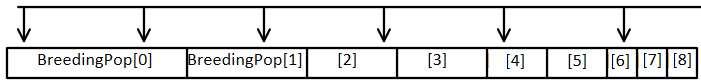
\includegraphics[width=0.7\linewidth]{figures/png/RUSIllustration}
	\caption[Roullete Uniform Selection]{An example of RUS. The bar represents the cumulative fitness of the population. The arrows represent which members of the population go on to become a breeding member.  In this example, 3 gets skipped even though it has higher fitness than 4 and 6, while 0 gets copied into the breeding population twice.}
	\label{fig:rusillustration}
	
\end{figure}
\\
With a breeding population in place, we can begin the breeding process.  This is typically accomplished via an operation called crossover, which I will explain below.  \\\begin{tabular}{c|c|c|c|c|c|c|c|}
	\textit{A} & \textit{1001} & \textit{10} & \textit{0011} & \textit{11} & \textit{1001} & \textit{00} & \textit{0111}\\ 
\textbf{B} & \textbf{0011} & \textbf{01} & \textbf{1000} & \textbf{01} & \textbf{0001} & \textbf{10} & \textbf{1001}\\
	
\end{tabular}\\
We begin with two solutions.  Crossover takes and returns 2 bitstrings.    It also has several subtypes, which I will illustrate in sequence.  First is one-point crossover.  This means that before crossing, a crossover point is chosen and offspring are produced as a copy, and when this point is reached, the offspring cross over and begin taking material from the other parent.  \\

\begin{tabular}{c|c|c|c|c|c|c|c|}
	\textit{A'} & \textit{1001} & \textit{1}\textbf{1} & \textbf{1000} & \textbf{01} & \textbf{0001} & \textbf{10} & \textbf{1001}\\ 
	\textbf{B'} & \textbf{0011} & \textbf{0}\textit{0} & \textit{0011} & \textit{11} & \textit{1001} & \textit{00} & \textit{0111}\\
	
\end{tabular}\\

Two point crossover is similar to one point, except that crossing happens twice.\\

\begin{tabular}{c|c|c|c|c|c|c|c|}
	\textit{A'} & \textit{1001} & \textit{10} & \textit{00}\textbf{00}  & \textbf{01} & \textbf{0001} & \textbf{10} & \textbf{1}\textit{111}\\ 
	\textbf{B'} & \textbf{0011} & \textbf{01} & \textbf{10}\textit{11} & \textit{11} & \textit{1001} & \textit{00} & \textit{0}\textbf{001}\\
	
\end{tabular}\\

Notice that here the final digit of A' and the second digit of B' becomes invalid (1111 is not between 0000 and 1001)- this is not controlled for in Crossover, but rather handled later by evaluating the offspring.

The final standard type is uniform crossover, which makes a check at each bit to crossover.  It results in much more mixing, depending on the probability of a crossover event.  One advantage is that it treats the beginning and end as the same, which can't be said for either of the first two.  Another is that it allows the designer to specify, directly and exactly, how much gene mixing should occur on average.

One thing that might be noticed is that regardless of where the crossover point is, with these methods if both A and B contain a particular bit in the same location, it will appear in both offspring.  This is one reason that diversity is important- if the population becomes too homogeneous, it will be unable to change except through random mutation, which we discuss shortly.\\
One other form of crossover we will deal with is one that counters this potential vulnerability.  It is a shifted crossover, so that one bitstring shifts forward a random number of bits, and then crossover proceeds normally.
\\
Other forms of crossover are possible, though they are not as widely represented in the literature.  One is a modified uniform crossover that checks to cross only  at each "word", that is at each column representing a digit or operator in our example.  This gives the designer some control over how much contiguous information is exchanged per crossover.  Other variations with three or more parents, or even random asexual reproduction are possible.  Logical operations are viable, though again care must be taken to not increase homogeneity overmuch. \\

\subparagraph{Mutation}
Mutation is fairly straightforward.  Usually after crossover and before insertion in the next generation, that is, only affecting the offspring of breeding and not elitism, each bit in the bitstring has a chance to change.  The algorithm is perhaps the most instructive: \begin{lstlisting}
for (Solution s in Crossover(A,B)):
	for each bit in s.Bits:
		if(MutationChance > Random(0,1)) bit = !bit
	end for
end for
\end{lstlisting}
There are some implementations that vary in that they will change random values to 1 or 0 rather than flipping bits (in other words, values will change about half as often).  A standard value for mutation is small, about 
${\frac{1.0}{Solution.Length}}$ which means on average 1 bit will change per solution per generation.\\
What is less straightforward are the effects of mutation over a population.  While values of 0 often stagnate in local minima, an upper correlate doesn't seem to exist- one could set mutation high, say 25\%, and turn off crossover entirely, and proceed with elitism and mutation alone and arrive at solutions.  In practice, this is much slower than using crossover. A general rule of thumb is to keep mutation low, and increase it even more slowly to combat stagnation.\\
\paragraph{Drawbacks}
While GAs have great versatility, there are some drawbacks which significantly limit their utility.
\subparagraph{Swiss-Army Chainsaw}
First, GAs are not the perfect solution for anything.  At their core, they are a biased-walk\footnote{With a random-walk on one side of the spectrum and a guided approach on the other.}.  This means that while they will come to a local optima, there is no guarantee they will achieve a global optimum.  If there exists a tailored solution for a problem, using that will probably work faster and better.
\subparagraph{And Quick to Anger}
Second, GAs are subtle things.  The fitness function, not given its due in this writeup, can be the difference between a quickly converging solution and processors spinning their wheels for days or months coming to one sub-satisfactory solution after another.  A GA will optimize the fitness function- and that's all it will do.  So if you want to maximize a metric, say accuracy for a classifier, be aware that it might do exactly that by simply guessing the most prevalent answer in the dataset.  This will get it to a local optima, and it might be surprisingly difficult to get it out of it.\\
Furthermore, there are hyperparameters which effect the GA directly but can be difficult to tease out.  What should the elitism percent be?  It probably depends on your other parameters.  There are ways of optimizing these, and they themselves might be amenable to a further GA, except that evaluating them is time consuming- should your fitness function be speed of convergence?  Or the best solution arrived at within 100 generations?  That might seem too long, but use fewer generations and you run the risk of invoking too much sensitivity to starting conditions to draw meaningful conclusions.  There are some rules of thumb to assist with these situations, but they only mitigate the problem, they don't eliminate it entirely.
\subparagraph{Toolset}
Finally, a GA is only as good as its toolbox.  On Earth, that toolkit was physics.  All of physics, and massively, embarrassingly parallel at that.  That's difficult to take advantage of digitally, where you not only have the responsibility of developing an encoding but also defining the universe your population lives in.  For instance, the heart of this paper is whether to use a GA to optimize a classifier or to use a GA to classify things.  The classifier has theory underpinning its toolkit, the GA has only whatever fitness function and encoding it is supplied.  Or, to get back to our example, it might speed convergence to increase mutation rates and restrict crossover to occur only at the breakpoints of binary words.  The downside of this is that GAs are supposed to be able to solve any problem, and while they can, they also require a certain amount of customization to not waste everyone's time.  The harder the problem, the more customization that is usually required.  And at that point, if a tailored solution of some kind exists it's probably easier to code up and implement than an equivalent GA.  At their core, the GA is a biased walk, but building in paths will hopefully make that walk much quicker.
\paragraph{Theoretic Underpinnings}
Intuition is often insufficient for or even anathema to scientific inquiry, and so far that is all we have relied upon to understand why GAs work.  The Fundamental Theorem of Genetic Algorithms is used to explain much of it.  First, where we explicitly represent populations as collections of bitstrings, we may impose an additional ordering on them, the schema.  Returning to our example, consider the equations: \begin{align*}
3 \times 7 \times 3 + 5 &= 68\\
9 \times 7 + 8 - 3 &= 68\\
9 \times 7 + 6 \times 2 &= 75
\end{align*}  
These translate to the bitstrings
\begin{align*}
0\textbf{0}1\textbf{1-10-0111-}&1\textbf{0}-0011-00-\textbf{0}101\\
1\textbf{0}0\textbf{1-10-0111-}&0\textbf{0}-1000-01-\textbf{0}011\\
1\textbf{0}0\textbf{1-10-0111-}&0\textbf{0}-0110-10-\textbf{0}010
\end{align*}
Let's just assume that our x is close to, but is not 68.  Let's say it's 71.  This means that each of these bitstrings will have a relatively high fitness.  Specifically, the first two have a fitness of $\frac{1}{|71-68|}=\overline{.3}$ and the third has a fitness of .25.   However, a close inspection of all bitstrings side-by-side shows that they have a considerable amount of overlap.  All begin with odd numbers multiplied by seven, etc..  You can see the overlapping sections in bold- but pay careful attention to the long contiguous sequence.
Schemata are a way of considering a population theoretically.  A schema introduces a third character into the alphabet of bitstrings- an * indicating either 1 or 0.  Schemata are of any length, and may be defined by their offset and bitstring (their length may be obtained from their bitstring).  Thus, offset 0 and "***1-10-0111-**" is a valid schema which describes both solutions.  In fact, there is one schema that describes both strings, which is already represented by retaining the symbols where it is bold and replacing it with * where they don't match.\\It should be obvious that doing any calculations with schemata are infeasible, simply because for even short bitstrings, the possible schemata to describe the population increase exponentially. Let m be the length of a bitstring, and S be the set of schemata which can describe the population.  Then let \begin{equation*}
	|S|=\sum_{i=1}^{m}3^i(m-i+1) = \frac{3}{4}(-2m+3^{m+1}-3)
	\end{equation*}
While we could try to constrain this by only using the schemata that describe the currently existing population, that problem is also exponential, and potentially worse computationally, because any member of the population has $$\sum_{i=1}^{m}3(m-i+1) =\frac{3}{2}m(m+1)$$ schemata that describe it, but then these would need to be compared with the sets generated by all $2^n$ combinations of members of the population.\\
However, feasibility of computation aside, we can use this to gain a further and more formal understanding of how GAs function.\\
Informally, if we assume that schemata describe our population, whatever they may be specifically, we may also assume that short, more fit schemata will have a greater than average fitness than is represented in the population, and as such these short, fit schemata are likely to increase in representation throughout the population.  Shorter schemata will survive because longer schemata are more likely to be broken up by crossover. 
Three more concepts need to be understood before the equation itself: First,  is the order of a schema H, which is the number of non-wildcard bits it contains.  Higher is more specific.  Second is the defining length, which is the distance between the first and last non-wildcard bits.  If we return to our example, and let $\schemaSymbol_a$= offset 0, "***1-10-0111" and $\schemaSymbol_b$= offset 0, "*0*1-10-**11", then $\schemaOrder{\schemaSymbol_a} = \schemaDefiningLength{\schemaSymbol_a}=7$, while $\schemaOrder{\schemaSymbol_b} = 6$ and $\schemaDefiningLength{\schemaSymbol_b} = 8$.  Third is $\schemaFitness{\schemaSymbol}$, which describes the average fitness of a schema.  This is defined as 
$$\schemaFitness{\schemaSymbol}=\sum_{s\epsilon \schemaAsFunction{P}}^{}\frac{\fitnessFunction{s}}{|\schemaAsFunction{P}|}$$ where H(P) is the schema H applied to the population P, which returns a subpopulation of solutions, and where s is one such solution returned.
   \\With these concepts understood, the Fundamental Theorem of Genetic Algorithms is as follows: \begin{align}
\schemaRepresentation{H}{t+1}&\geq \schemaRepresentation{H}{t} \frac{\schemaFitness{\schemaSymbol}}{\averageFitness}\bigg[1-\bigg(\crossoverRate+\schemaOrder{H}\mutationRate\bigg)\bigg]
\end{align}
Where $\averageFitness$ is the average fitness of the population at time t.  $\crossoverRate$ and $\mutationRate$ are probabilities of crossover and mutation, respectively, and $\schemaRepresentation{H}{t}$ is the number of representations of a schemata H at a time step t in a population.  The type of crossover plays a role, here.  Depending on implementation, in single point crossover the probability of crossover occurring is usually 1.  Instead, a random number from 1 to L is usually chosen, with each index being equally likely, and crossover occurs at that index. Thus, for single point crossover, $$\crossoverRate^{SinglePoint} = \frac{\schemaDefiningLength{H}}{L-1} $$ For two point crossover, the odds of breaking a given schema is much more likely, because it is the outcome of 2 events not happening, that is $$\crossoverRate^{TwoPoint} = 1-\frac{L-\schemaDefiningLength{H}}{L-1} \frac{L-\schemaDefiningLength{H}}{L-2} $$ from which we get the general $$\crossoverRate^{NPoint} = 1- \frac{(L-\schemaDefiningLength{H})^n}{\frac{(L-1)!}{(L-1-n)!}} $$
for n point crossover. \\Uniform crossover is implemented differently, and is generally done with a rate, which we'll call $\gamma$.  Since this is the case, it makes calculating $\crossoverRate$ more straightforward.  
$$\crossoverRate^{Uniform} = 1 - \gamma^{\schemaOrder{H}} $$So, while representations for schema which are more fit than others will increase over time, the particular type of crossover can have a significant impact on how much representation they gain.  It is worth noting that a uniform crossover with even a moderate rate of crossover (say, .3) can rapidly lead to the eradication of all higher-order schemata.  Also worth noting is that when a schema applies to both solutions, both offspring will also belong to that schema using standard crossover methods.  Finally, if an implementation includes a probability other than 1 for any of the forms of n point crossover, that probability is simply multiplied to the appropriate $\crossoverRate$.\\
A few observations about this function.  As overall length of the bitstring increases, the inhibition of single-point crossover decreases, but inhibition of n point crossover generally increase, and if the mutation rate is linked inversely to length then it does as well.  Uniform crossover is less directly linked to length, though not independent: as L increases, the numbers of higher order schemata increase exponentially.  Survival of a particular schema becomes very unlikely without a strong selective pressure toward retention. Further, high order and fitness schemata with greater defining lengths rapidly become unlikely to obtain except through elitism.  
\\
\paragraph{Motivations}
Over the course of researching how GAs were being used in recent times a broad pattern emerged.  With regards to classification, there were two basic schools of thought:  one in which GAs were used to optimize classifiers and one which used GAs as classifiers directly.  Both camps have \textit{prima facie} impressive examples of these approaches.  Thus, this project was born- to attempt to answer which approach is more generally applicable.\\
GA are widely used for numerous purposes, but we seek to ascertain their suitability for pattern recognition, specifically classification.  In this paper, we attempt to determine how suitable GAs are for the task of classification.  To determine credibility, we propose 3 tests.  First, we will run a GA on the datasets acting directly as a classifier.  Second, we will run two classifiers, a lone Decision Tree, and a Naive Bayes classifier with default settings as a control.  Finally, we will run the same classifiers optimized through a GA which will run for a modest number of generations.  We will collect confusion matrices from the resulting classifiers and compare them.\\
To ensure that our approach is generally applicable, we propose datasets from divergent fields of study and with data in different configurations.  With minimal adjustments, the program we have written is capable of automating this process over almost any dataset, but we have chosen 3 from the UCI repository\cite{lichman_uci_2013} : Yeast Dataset (Yeast)\cite{paul_horton_uci_1996}, Bach's Chorales Dataset (Bach)\cite{daniele_p._radicioni_uci_2014}, and Cardiotocography Dataset (Cardio)\cite{j._p._marques_de_sa_uci_2010}.  This gives us 4 different configurations to use, as Cardio has two modes that it runs in, with the pattern class code (1-10) or the fetal class code (Normal, Suspect, Pathologic).  This gives us data from biology, music, and medicine, which serves as a broad start.  However, we are also making the code available in in its entirety for anyone who wants to extend this to other domains of study.\\
\subparagraph{Priors}
Going into this project, a case for either side could be made.  On the case for the Pure GA approach you have a few points.  First and foremost versatility- the GA is only limited by the encoding, and a clever encoding could exploit nuances that people wouldn't be likely to notice in the data.  Secondly, there's something about the simplicity of only having 1 component to debug- this could speed development which would mean more effort could be spent developing the encoding and the fitness function.  One con is the inverse of the first pro- that encoding needs to exploit the nature of the data, and so much time can be spent customizing the approach to the data, but this is also antithetical to the idea of a generic solution to classification, so whatever encoding we use must be good enough to apply to many problems.\\
For the Hybrid camp, the pros are primarily that the GA gets to leverage the theoretical robustness of the external classifier.  That is to say that there has been a great deal of work to make classifiers extremely good at what they do- and writing a GA to compete with or exceed beyond that work is difficult.  There are several cons, though- the external classifier needs to be written and debugged separately and then in conjunction.  Also, there are now 2 or more entities to be maintained which means much less time can be spent on any one project, unless you simply tie into some other classification package, though that may have its own challenges.\\
Thus, before going into this project, we slightly favored the hybrid approach.  But we wanted to make sure that there was plenty of versatility for the GA to make use of, so for the implementation of our pure GA we settled on CellNet \cite{kharma_project_2004}, which is a variable length GA which has a new breeding operator.  We discuss this project in depth in Chapter 2.  

\paragraph{Literature Review}
\subparagraph{Hybrid Approach}In \cite{schuman_spatiotemporal_2014} they use classifiers to breed numerous neural networks in parallel and test them against MNIST.  In \cite{ocak_medical_2013} the authors use a support vector machine (SVM) optimized by a GA to predict fetal well-being, with considerable success.  In \cite{marchetti_improving_2013} GAs were used for feature selection and then the features generated were passed to a logistic regression classifier.   In \cite{wu_evolving_2015} GA were used in conjunction with particle swarms to optimize a neural network for predicting rainfall.  While GAs performed better in conjunction with the particle swarms than alone, the idea of using a GA to build a better classifier is present.  \cite{chou_optimizing_2014} and \cite{duan_characterization_2014} discuss using a GA to optimize another SVM, this time emphasizing the mileage obtained from leveraging the SVM for curve fitting while the GA handles the optimization of the SVM itself.  \cite{devos_simultaneous_2014} takes a similar approach, but instead focuses on using the GA to determine which combination of preprocessing methods to use.  The GA is also used to determine two meta parameters for the SVM itself.  Once these are determined, the SVM is used to handle the classification.  In \cite{uysal_text_2014} they use GAs to focus their Latent Semantic Indexing approach on promising semantic features.  They use two different approaches and find that both are much more effective on a wide range of tests than the approach without the GA optimization. \cite{salari_novel_2014} used an ensemble approach which is quite novel.  First, they use doctors to decide which features of the datasets in question to use.  Then, they give these features to a Feed Forward Neural Net(FFNN) on one hand and a GA on the other.  The GA generates several different arrays of features, and then these arrays and the results from the FFNN are fed to a k nearest neighbor to find fuzzy classes, then those classes are iteratively pared down until they are no longer fuzzy.  They apply their model to multiple datasets, and compare across a wide variety of methods with a variety of metrics, over which they show statistically significant gains on nearly every method, metric, and dataset.  \cite{alexandre_hybridizing_2015} hybridizes a GA with an Extreme Learning Machine, with considerable gains in both binary and multiple class classification over multiple learning methods.


\subparagraph{Purist}
Here, we look at papers where GAs act directly as the classifier.  We have included papers where rules for classification are generated.  \cite{dehuri_application_2008} uses two different GA approaches to classification rule generation, one a simple one similar to the "canonical" approach and one a multi-objective optimizer.  The multi-objective GA performed well, though areas for improvement were discussed in the conclusion.  One area particularly limiting the GA was the number of attributes the GA was working with.  The interestingness of the discovered rules was quite high, though sometimes the comprehensibility was lacking.  Still, the rules were highly predictive on the datasets employed.
In \cite{kozeny_genetic_2015} they used 3 GAs to calculate credit scores, and compared their accuracies.  While they achieved interesting results with their methods, the most promising one scales a $O(2^L)$, which makes it unfeasible except for short feature sets.  In \cite{srikanth_variable-length_1995} variable length GAs are used to draw fuzzy ellipses in a decision space, and thresholding is used to make the borders crisp.  This approach is shown to be comparable over their selected dataset to a back-propagation neural net (BPNN).\\
\cite{fidelis_discovering_2000} uses a GA to develop rules for diagnosing breast cancer and dermatology.  They achieve 95\% accuracy on the dermatology but only 67\% on the breast cancer- which is, by the author's own admission, a much more difficult dataset with a great deal more noise.  Beside the results, the rules themselves were of interest, and evolved 3 separate times from different random seeds.   The rules themselves seemed to hit the knowledge discovery trifecta of predictiveness, comprehensibility, and interestingness.\\
In \cite{hoque_implementation_2012} and \cite{li_application_2012}, GAs are used to solve an intrusion detection problem.  While both papers boasts a discovery rate of nearly 100\%, if one ignores the denial of service attacks their discovery plummets.  Unfortunately, it isn't clear that the authors are entirely at fault for this- the data used for the DARPA challenge contained 5,283 non-DoS attacks, but 391,000 DoS attacks (it also contained 97,000 non-attacks).  It’s small wonder that the GAs would optimize according to this aspect of the data.
\cite{tseng_genetic_2008} is another example of rule discovery, but this time applied to land-cover classification.  They specifically use a GA as an alternative to other methods such as a Neural Net(NN) or other Bayesian classifiers because the GA has shown that the rules it discovers are more comprehensible, even if less predictive.  In other words, while NNs may be good at solving a problem, exactly how they solve it is not always clear, and that can be problematic for many domains.  Unfortunately, while they get good accuracy they don't do a head-to-head comparison.  One possible reason is because the database is very small, at only about 400 samples.\\
Finally, and we will discuss the  inspired CellNet family of papers in much more detail in Chapter 2.  However, in the original \cite{kharma_project_2004} CellNET paper, they used a variable length GA to classify the \cite{cedar_cedar_2002} database.  While they obtained modest results, the stated goal of CellNet was to develop a GA which could approach any dataset with minimal intervention.  They continued in \cite{kowaliw_cellnet_2004}, where they employed two populations of competitive solutions called hunters and prey, where hunters are trying to classify a handwritten digit from the CEDAR database and prey are trying to obscure said image.  The results in this paper were much more impressive, and their overfitting problem diminished significantly as well.
\pagebreak

    \chapter{Methods and Implementations} \label{ch:Methods}
\section{Overview}
In this chapter we'll discuss the design decisions we've made in detail.  We
have 3 distinct phases.  The first phase, preprocessing, is converting the data
files into a unified dataset in memory and configuring for the following phases.
The second phase is the hybrid approach where we optimize external classifiers,
followed by the purist approach where we use our genetic algorithm (GA) to
develop classification rules.  Each of these approaches generate confusion
matrices which we analyze.\\
The general flow of the algorithm can be seen in \ref{fig:ProgramFlow}. 
\begin{figure}
	\centering
	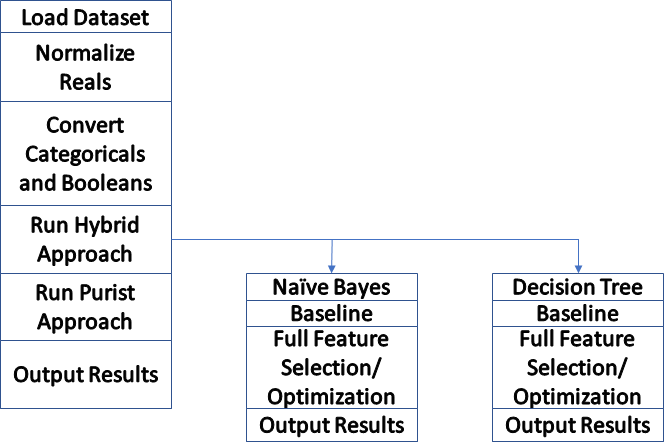
\includegraphics[width=0.7\linewidth]{figures/png/ProgramFlow}
	\caption[Overall Program Flow]{Birds-eye view of the flow of the program.
		Hybrid approaches are not run in parallel, because at time of coding MATLAB
		doesn't support multi-threading via a COM server.}
	\label{fig:ProgramFlow}
\end{figure}
Loading and normalization gets all algorithms on the same page, ensuring an
apples-to-apples comparison.  First we have the hybrid approaches.  Within a
hybrid approach, we first see what optimizing without including features yields-
this is referred to in the code and in the program as the hybrid approach.  It
has all the same constraints as the parent approach.  After the baseline, we
optimize a second time, this time including feature selection, by which we mean
that we characterize a dataset with n variables as either included (1) or
excluded (0) in a bitstring, and encode the same variables to the classifier as
in the baseline method.  We have selected two distinct classifiers: a multiclass
na\"ive Bayes algorithm and a simple single decision tree.  Each of these are
run twice per dataset- once with feature selection disabled (the baseline) and
once with it enabled.  We will discuss those methods in more detail in their
respective sections.\\The purist approach is much more straightforward.  There
is only one mode which it runs in, there's no explicit feature selection.  That
is, there is feature selection, but all features are available to the algorithm
at any time- just some may or may not be included. This portion of the algorithm
is threaded.  
\section{Preprocessing}
We do some preprocessing of the data.  First and foremost, there is a text file
that is read which describes the dataset and points to where it is on the
filesystem.  Below is an example- this tells the program where it can find X and
Y and how to parse them.\pagebreak
\begin{lstlisting}[language=config, caption={Cardio Config File}, label={fig:config}]
#Dataset Name
CardioData
#Class Names File
../../../Data/Cardio/classNames.txt
#TrainingSet X Path
../../../Data/Cardio/trainingXY.csv
#TrainingSet Y Path
../../../Data/Cardio/trainingXY.csv
#TestingSet  X Path
../../../Data/Cardio/testingXY.csv
#TestingSet  Y Path
../../../Data/Cardio/testingXY.csv
#X ignore list, comma separated and starting with w if it's a whitelist
(otherwise, blacklist)
b, 29, 30
#Y ignore list, as above
w, 29
#Categorical Variables, white/blacklist, comma separated
w, 
#Boolean Variables, as above
w, 
\end{lstlisting}

For instance, in this case X(the data) and Y(the labels) are in the same file,
but represented as different columns.  They could easily be stored as two files.
After those files are explained, the next uncommented line describes the
columns to ignore or include, specified with b for blacklist or w for whitelist
respectively.  In this example, columns 29 and 30 are ignored for X, but only 29
is included for Y.  This is because for this dataset, there are two sets of
labels and thus two separate description files to use the file differently. 
Using the same notation, we can declare categorical and boolean variables for X.
Y is assumed to be categorical.\\
After we read how to parse the file, we read the files themselves.  At this
point we also convert booleans and categorical variables to doubles so that they
can fit in the same matrix.  First, however, we want to normalize the Reals. 
First we gather max, min and mean from each column in the dataset.  Then we use
a function to squeeze the values down between .1 (b) and .9 (t) for reasons that
will be seen later in the section on the purist approach.  
$$x_i^{\prime} = b+(b-t)\frac{(x^i-x_i^{min})}{x_i^{max}-x_i^{min}}$$ Next,
categorical variables are given the treatment motivated and described fully in
\cite{zhang_visual_2015}, the conclusion being that every category label is
replaced with a real number which maximizes Pearson's Correlation Coefficient. 
That is,
\begin{align*}
X &= {X_\mathbb{R} \cup X_{cat} \cup X_{bool}}\\
X_\mathbb{R} &= \{x_1, x_2, ... x_n\}\\
X_{cat} &= \{x_1, x_2, ... x_c\}\\%there are some number of categorical columns,
%each of which have a number of categoricals in them.
X_{bool} &= \{x_1, x_2, ... x_b\} \\
1&\leq i \leq c\\
L &= \{x_i|x_i\epsilon X_{cat}\}\\%Set of categoricals
C_l &= \{x, i|  x\epsilon X \wedge x_{n+i} = l\epsilon L \}\\%set of samples
%belonging to categoricals
\end{align*}
Where X is the dataset, $X_\mathbb{R}$ is the real portion of the dataset, and$
X_{cat}$ and $X_{bool}$ are the categorical and boolean portions.  The index i
iterates over the columns of $X_{cat}$, which lets us derive L, which is the set
of all categories in the dataset.  L in turn gives us a means of devising $C_l$,
that is, the subset of X which consists of all members of x which belong to the
category $l$. Now it is possible to look at $C_l$ and determine which values
will maximize $r^2$ for each label l, which we here call R(l).
\begin{align}
R(l) &= \frac{\sum_{x\epsilon C_l}\sum_{j=1}^{n}x_j}{|C_l|n}
\end{align} 
It can be seen as the mean of all the other values over $C_l$.  Calculating this
in practice is much more straightforward- simply step through X one sample at a
time, and maintain running sums and counts for each unique label, calculate the
means at the end and then extend $X_\mathbb{R}$ with the newly calculated
values.  In the case of multiple categorical columns, unless there is a perfect
correlation between two category labels each label will have its own value
(though this can't be proven to be unique, only generated from a unique set of
numbers).\\
Booleans are only given the treatment of being converted to values .25 for false
and .75 for true.  Again, the reasons we don't use 0 and 1.0 will be made clear
in the section on our purist approach.\\
Now that the data has been modified, some additional bookkeeping is
accomplished.  Conversions to numerics from string class labels and vice versa
are computed and stored, since mathematical approaches prefer integers while
human-readable outputs are in the terms given us by the dataset.  Also, global
values such as Elitism Percentage and Population Size are modified at this point
and are effectively constant for the rest of the program.  Variables that may be
configured by the user are: Max Generations, Record Interval, Population Size,
and Complexity bounds.  The Max Generations sets the stopping condition of the
algorithms, and defaults to 100.  The Record Interval determines how often to
save data to the disk- data is collected every generation, but is only saved to
disk in where $G mod(RI) = 0$, and the default is 25.  Complexity bounds are
discussed in more detail in the purist approach, and have no effect on the
hybrid approach.  Other modifications to semi-constants are made at this point
determining the length of chromosomes for both approaches based on the
characteristics of the datasets- particularly the number of features.
\section{Hybrid Approach}
As mentioned previously, the hybrid approach consists of 2 methods which each
consist of two different ways of running them.  First we will discuss the
multi-class na\"ive Bayes (McNB) approach, followed by the decision tree (DTree)
approach.
\paragraph{McNB}
Na\"ive Bayes is one of the most basic of classifiers, but it is powerful and
versatile.  Without going into extreme detail, it generates probability
distributions for each class across every dimension in the feature set from the
training data, and picks the most likely class for a given sample point. 
Typically, the probability distributions are Gaussian, however any density
function can be used.   We use this because it should provide a fairly low bar
to compete with- support vector machines (SVMs) are much more complex, tend to
be extremely reliable and robust, and are close to something resembling the
industry standard, but don't perform well with multiple classes.  McNB is closer
to statistical modeling and is not what we consider machine learning, though no
bright line distinction exists.  It is a theoretically grounded but simple
statistical method well suited to being a first pass at the data or being used
in conjunction with other methods.  Being simple, it is also relatively fast-
only 2 passes through the data are necessary to build the parameters for the
PDFs, so building the model can be done in linear time.  Once built, checking a
given variable can be done in constant time.
\begin{equation}
P(A|B) = \frac{P(B|A)*P(A)}{P(B)}
\end{equation}
The standard formulation of Bayes' theorem, in our case it is more useful to
form it thus:
\begin{equation}
P(\omega_j|x) = \frac{p(x|\omega_j)P(\omega_j)}{p(x)}
\label{eq:bayes}
\end{equation}
Here, $\omega_j$ is the likelihood of belonging to a particular class.  Upper
case $P$s are simple probabilities, lower case $p$s are more complex functions.
So $p(x|\omega_j)$ is the PDF, and $P(\omega_j)$ is the prior, which can be
thought of as \textit{a priori} how likely a particular class is to present.  To
build the PDF, if we're using a Gaussian, we need mean and standard deviation
for each class.  The Gaussian PDF is built using the training set, tested on the
testing set, and the results are scored in a confusion matrix.  This can be
determined from the dataset, in which case it uses the frequency in the Training
set to generate priors, or set manually.  In either case, this can be seen to
scale a particular PDF.  In fact, this is similar to what $p(x)$ does- except
that where $P(\omega_j)$ scales a class, $p(x)$ scales all classes, and it
serves as a normalizing factor to constrain values between 0 and 1.  It could
be established using the law of total probability, or it could be some
arbitrarily high constant\footnote{It doesn't really make a difference, since the selected class will just be the one with the highest score given x. 	Furthermore, if it affects all classes equally nothing is served by making
complex calculations every time the classifier is called.  Simply calculate the highest value it could take initially and use that in subsequent calls.}.  \\Our implementation, which we'll refer to as the McNB optimizer\footnote{To avoid confusion, our optimizers are optimizing classifiers, they are not classifiers but optimizers.  Later, we present our classifier.} optimizes the fitcnb  \footnote{For much further
detail on Mathworks' implementation see
\url{http://www.mathworks.com/help/stats/fitcnb.html}.   function in MATLAB over the following parameters: distribution, kernel, score transform, and priors.  Further, it optimizes over the dataset by choosing which features are included.  It is entirely defined by its bitstring, the first several bits correspond one-to-one to the features in the dataset.  An optimizer with all 1s (or all 0s to avoid having no data) will include the entire dataset.  Otherwise, a 1 indicates that the column is included, a 0 removed.
}  \\
The distribution uses 2 bits and can be any of the following values:\\
\begin{itemize}\item Kernel uses a smoothing function, described below.\item
	Multinomial represents every class as a single multinomial distribution.\item
	Multivariate multinomial characterizes each feature as an independent
	multinomial distribution based on the unique values found in the feature.\item
	Normal distributions behave as described above.
\end{itemize}
Kernel type uses two bits, though these go unused unless the the distribution is
kernel.  Then the variables are smoothed via various functions outlined below.
\begin{itemize}
	\item \textbf{Box} uses a uniform, box-like smoothing window.
	\item \textbf{Epanechnikov} is a very efficient, rounded kernel.  Minimizes
	Asymptotic Mean Integrated Square Error (AMISE)\cite{stefanie_scheid_introduction_2004} therefore optimal
	in that sense.
	\item \textbf{Gaussian} is a standard normal function but used in this case for
	smoothing.
	\item \textbf{Triangular} is another form of smoothing, with a peak of 1 at 0
	and zero at -1 and 1.
\end{itemize}
Regardless of which form of smoothing, the goal is the same- to create a
distribution of a random variable which can then be modeled.  This is done using
something like a histogram, which is then smoothed into a continuous function
using the kernel chosen above.  This becomes $p(x|\omega_j)$ in the equation
\ref{eq:bayes}.\\
For priors, each class extends our optimizer's bit length by 3 bits.  Each class
then has a prior of $(1 + 0-8)= 1-9$ which is later summed and turned into a
probability distribution summing to unity.  For instance, if there are 2 classes
and one has a prior of 3 while the other has a prior of 7, these are converted
into percentages of 30\% and 70\%, respectively.  These become the $P(\omega_j)$
in equation \ref{eq:bayes}.\\
Finally, the score transform takes up 3 bits and can be any of eight values. 
This is used internally in the MATLAB function.  It can be any of the following
values:
\begin{itemize}
	\item DoubleLogit transforms the score to $\frac{1}{1+e^{-2x}}$
	\item Invlogit $log(\frac{x}{1-x})$
	\item Logit $\frac{1}{1+e^{-x}}$
	\item None $x$
	\item Sign $\frac{x}{|x|}$, or 0 when x = 0.
	\item Symmetric $2x-1$
	\item Symmetricismax 1 if max of class, 0 otherwise
	\item Symmetriclogit $\frac{2}{1+e^{-x}}-1$
\end{itemize}
Once these are determined, the optimizer is evaluated.  This means that the training set is passed to the optimizer, it is trained, and then the testing set is passed to it, from which we get the fitness of the classifier.  Fitness is average accuracy.  That is, suppose we have a confusion matrix C\\
C= \begin{tabular}{|c|c|c|c|c|}
	\hline
	True:&$\omega_1$&$\omega_2$&$\omega_3$&\textbf{Total}\\
	\hline
	Predicted $\omega_1$&4&2&5&\textbf{11}\\
	\hline
	Predicted $\omega_2$&2&2&5&\textbf{9}\\
	\hline
	Predicted $\omega_3$&8&6&110&\textbf{120}\\
	\hline
	Total&\textbf{14}&\textbf{10}&\textbf{124}&\textbf{144}\\
	\hline
\end{tabular} 
\\The dataset in this case has 3 classes, $\omega_1$, $\omega_2$, and $\omega_3$, and has 144 total samples.  Of those, 14 are class $\omega_1$, 10 are class $\omega_2$, and 120 are class $\omega_3$.  Meanwhile, the classifier predicted that 11 of the samples were $\omega_1$, 9 were $\omega_2$, and 124 were $\omega_3$.  To determine accuracy, the equation is $\frac{\sum_{i=1}^{3}C_{ii}}{144}$.  This is a good metric for relatively evenly distributed classes.  However, in highly skewed cases as this one, this treats more rare classes as less important.  For instance, in this case, the accuracy is $\frac{116}{144} = .805$, which might seem like it is doing a decent job, and maybe it is, if the concern is finding Cs.  Average accuracy is slightly more complicated to calculate, but still straightforward enough.  First, lets define the Total column more formally: $$T(\omega_i)=\sum_{j=1}^{N}C_{ij}$$
Where N is the number of classes.  Thus, average accuracy, $\overline{A}$ can be defined as $$\overline{A} = \frac{\sum_{i=1}^{N}\frac{C_{ii}}{T(\omega_i)}} {N}$$
In our example, $\overline{A}$ is .467, which seems more like the classifier is doing barely better than chance.  In fact, if it had just guessed everything was $\omega_3$, accuracy would be higher (.833), but $\overline{A}$ would have been .333.  Further, $\overline{A}$ is equivalent to accuracy if all classes are equally distributed, thus there is no disadvantage to using it.  Average accuracy is a major factor to the fitness functions used in this project.\\
We will next discuss another type of optimizer, and then we will discuss what they have in common.

\paragraph{CTree}
Decision Trees are an algorithm which take a dataset and make usually boolean decisions from its features, which generates a hierarchy resembling a tree.  They are very easy to compute, but usually aren't the most robust of classifier unless used in ensembles.  However, finding an optimum decision tree has been shown to be NP complete \cite{hyafil_constructing_1976}, so greedy approaches are often used to approximate the perfect tree.  Decision trees are referred to as Classifier Trees or Regression Trees, depending on their task.\\
Decision trees are typically generated using a greedy algorithm to maximize the split criterion at each of several splits.  The Gini impurity is $1-\sum_{i}p^2(i)$, where $p(i)$ is the fraction of samples belonging to $\omega_i$ which reach the node.  It is distinct from the Bayesian prior because it doesn't apply equally to all samples.  For instance, there might be 10 classes in a dataset, but if only one class would reach a node, then the sum of $p(i)$ would equal 1, and the Gini impurity would be 0. Thus, it can also be seen as the probability of \textit{misclassifying} a sample based on the distribution at that node. Gini impurity is maximized as every decision, insuring that nodes are diverse.  There is often a limit to how deep the tree can get, that is the maximum number of decisions can be made for any given sample.  Gini impurity is closely related to entropy, and some decision trees are implemented using information gain instead- however, the difference in output is minimal, while Gini is marginally easier to compute.  For completeness, entropy of a node may be defined as $E=-\sum_{i}p(i)log(p(i))$ and it is possible to use entropy gain as the split criterion.  A third criterion is twoing, which is quite different.  It tries to find a division of samples whose class makeups are as homogeneous as possible and also make close to 50\% of the samples at the node the node, and then it tries to find a split to make that grouping possible.  For instance, if 4 classes were at a node, and two of the classes made up 50\% of the samples at the node, the algorithm would try to find a split that would maximally separate those two classes from the others.  
\\
The next optimizer we'll discuss is the Classifier Tree (CTree) optimizer.  This is optimizing MATLAB's fitctree\footnote{See \url{https://www.mathworks.com/help/stats/fitctree.html} for examples and further details.} function over the following fields: Merge Leaves, Maximum Splits, Min Leaf Size and Split Criterion.  Each CTree optimizer is completely defined by their bitstring, which are typically much shorter than for McNB.  It too begins with a representation of the features in the dataset, 1s for included, 0s for excluded, and either all 1s or zeros mean the entire dataset is included.  \begin{itemize}
	\item \textbf{Merge Leaves} takes 1 bit and is either on or off.  Merge leaves looks at leaves from a parent node and if the amount of their risk (a term which we believe corresponds to Gini impurity, but we can't find sources backing that up) and that of their offspring is at or greater than that of a parent.  In our CTree optimizers, this takes up one bit of the bitstring.
	\item \textbf{Maximum Splits} defines how many splits a tree can have.  The tree is built iteratively, layer by layer, splitting as needed until it hits this number.  In our optimizers, 6 bits are reserved for it, yielding values of 3-66.
	\item \textbf{Min Leaf Size} This is the minimum number of samples that need to reach this node to be considered a standalone leaf.  Beyond this number (specifically, at twice this number) a leaf become a parent node split into two children.  Five bits are reserved for it, yielding values between 1 and 32.
	\item \textbf{Split Criterion} can take on 3 values.  Gini's diversity index as discussed above, twoing, and deviance.  When deviance is selected, the rule is maximally reducing deviance with every split (effectively using entropy rather than impurity).  With Twoing, it will try to make an optimally balanced tree, erring toward balance rather than composition (in practice, these tend to be similar to entropy based trees).  These take up 2 bits of the CTree optimizer's bitstring.
\end{itemize}
\paragraph{Optimizers}
Our optimizers use inheritance to share common code.  So both CTree and McNB use many of the same mechanisms when it comes to evaluation and evolution.  First, both of them use MATLAB as their engine.  Unfortunately, while support is planned for a future release, evaluations done through the COM server (as opposed to done through the MATLAB SDK and compiler) do not support multi-threading, so even if multiple threads were used in the native code, there would be no performance gains to speak of.  In fact, while we don't have metrics any longer, execution was considerably slower when we were using the multi-threaded model.  We did at one point make use of the MATLAB SDK to compile the MATLAB code into native, and this was indeed faster- but there's considerable overhead involved and unless you have a MATLAB educational license, considerable cost.  Thus we have opted for the sub-optimal but considerably more cost effective implementation.\\
There are many commonalities.  For instance, initialization of a new Optimizer is really only dependent on the length of that class.  The core mechanism is the same in both of these classes (and several others that we have implemented outside the scope of this thesis).  Also, once an Optimizer is initialized, there may be errors.  While the concrete classes can handle the details, in the abstract the general principle holds that once an Optimizer is initialized, it needs to be prepared for evaluation.  For instance, if CTree's split criterion is 3, when only 0-2 are allowed, then those bits need to be rerolled.  The rerolling itself is common Optimizer code as are several utility functions, such as logical operators between two Optimizers.  \\
Scoring binary or multi-class Optimizers, saving them, much of the file IO, most of the life-cycle of an Optimizer, and memory management is handled in the common Optimizer code, meaning that implementing a new type of Optimizer can take a tiny fraction of the time implementing a new optimizer can- and even the MATLAB dependence is optional.  The relevant code is actually in the Globals file and the Eval functions in the concrete subclasses.  Optimizer does provide a virtual convenience method of ComEvalFunc which handles common cases, but there's no requirement for that to be called in a subclass.  The upshot is that this could be used with an entirely different sort of function- it wouldn't necessarily need to be a classifier at all\footnote{We plan on using this framework to experiment with integer Linear Programming in the future, for instance.}.  It could easily be sub-classed and modified to optimize different criteria altogether.  The other heavy lifter in terms of inheritance is done by Evolver.

\paragraph{Evolver}
Evolver is the class which makes up the bulk of the evolutionary algorithm.  Where Optimizer provides a framework for the finer details, Evolver handles the broad strokes of evolution.  It maintains a population of Optimizers and handles their life cycles in a way that is both extensible and straightforward.  \\This is in large part due to the fact that the evolution is entirely class-independent, implemented using templates. While it requires that the class being optimized is a subclass of Optimizer, that's really the only requirement; simply sub-classing Evolver and adding a new interface would allow dramatic changes to the function being optimized.\\First, let's look at our modified algorithm, as this will provide more details.
\begin{lstlisting}[caption= {Evolver Algorithm}, label = {fig:evolverAlgorithm}]
AdvanceGeneration():
	//P is the population and a class variable 
	EvaluateAllOptimizers(P)
	GetMetrics()
	P.ReverseSort()
	P = GenerateNextGeneration(P)
	RemoveDuplicates(P)

GenerateNextGeneration(P):
	BreedingPop := StochasticRUS(P)
	NextGen := Elitism(P)
	FillListFromBreedingPop(NextGen, BreedingPop, P.Count, UniformXOver)
	MutateNonElites(NextGen)
	return NextGen
	
FillListFromBreedingPop(N, B, size, Func):
	E := B.Count * ElitePercent
	while(N.Count < size):
		k := j := RNG.Next(0, E)
		while(j==k) 
			k = RNG.Next(0, B.Count)
		for each offspring in Func(B[j], B[k])
			N.Add(offspring)

	while (N.Count > size)
		N.pop()
	
\end{lstlisting}
So lets examine the high-points of these algorithms.  While EvaluateAllOptimizers might seem straightforward, in the details of that function we can either use multi-threading or not (we do not if we are using the COM interface to MATLAB), and we maintain a hash table of all tested Optimizers and their fitness, along with secondary characteristics if those are important.  This is from an earlier instantiation of our system where evaluation was extremely costly and so the extra overhead was worth it to save cycles. This is only possible because performance is entirely defined by the bitstring, this lets us test each string once and never test it again.  Finally, in FillListFromBreedingPop,  Func is UniformCrossover, but that's just one of several modules supplied.  In fact, as the signature is written\footnote{The signature is Optimizer[] BreedingFunction(Optimizer A, Optimizer B)- however, there is also a related function template provided which takes a variable number of parents.}, it could easily take any sort of two-parent breeding function, with any number of offspring.  Three or more parents could also be implemented if that was desired, though this would require sub-classing.\\
RemoveDuplicates is also important- any Optimizers that are removed are replaced with randomly generated new ones whose bitstrings are checked to be unique before replacement is finished, so the population size is maintained.  The reason this is important is because the breeding selection we're using in FillListFromBreedingPop is a variation of the Biased Random Key model \cite{ruiz_biased_2015} which provides great selective pressure but makes duplicates more likely as the elites become more homogeneous.  It is a modification because the model in the paper guarantees that every offspring will have at least 1 elite parent.  Our implementation doesn't, because we're drawing both parents from the breeding population and because of RUS there's no guarantee that any Optimizer other than the one at B[0] will be elite.  Instead, they are very likely to be elite.\\
The metrics we capture in GetMetrics are simply best and average fitness, but this provides an entry point to capture population metrics in a subclass or modification of the code.  In GenerateNextGeneration, we use RUS and Elitism as discussed in Chapter 1.  We also mutate the non-elites after our next generation has been determined.
\paragraph{OptimizerProgram}
There's only one more major component to the hybrid approach, and that is the OptimizerProgram class, which handles hyperparameters to Evolver.  How often to write data to disk, whether or not to multi-thread, population size, how many generations to run and file IO, as well as insuring all the directories for file IO exist are among the duties handled in this class.  Incidentally, we employ what we refer to as a baseline mode, which means running Evolver two different ways.  The baseline method runs Evolver with all columns turned on- in other words, it restricts the evolutionary process from functioning as a feature selector and only optimizes parameters to the classifier itself.  Then it runs again, this time without the restriction.  This provides a baseline comparison to see how much performance changed when feature selection is included in the optimization.
There are of course many, many more details in the code itself, which is available in the appendix, and comments provide motivation for much of the detail in situ.  This writeup should cover the high points, however, and give a reader an idea of what they are looking at in the code.
\section{Purist Approach}
In this section, we will discuss the implementation of a pure approach to classification.  Classification is executed by the evolutionary algorithm itself.  To understand all the parts working together, a bottom-up approach is instructive.  However, to guide that discussion, let us begin by motivating the algorithm.
For an evolutionary algorithm, we need a population of solutions to evolve.  In this case, we borrow the terminology and much of the methodology from \cite{kharma_project_2004} and say the population comprises Hunters, which are the form our solution will take.  While this paper may not be a perfect reimplementation of theirs, it is strongly inspired.  These hunters each have one or more chromosomes, which each have one or more cells.  Now we shall look in each component in detail.
\paragraph{Cells}
The cells are the fundamental building block of the hunter.  Each cell codes for a function, an upper and a lower limit, and a not flag.  Each cell has the ability to vote on a sample, which is an array of some number of doubles, each of which must be $\epsilon[0,1)$.  When a cell votes on a sample, it is equivalent to saying, "feature f is [not] between lower limit and upper limit".  Where not is the not flag, and feature f is a particular entry in the sample.  Lower and upper limits are each binary encoded reals, which use 8 bits each.  The encoding is straightforward- the bits have all been shifted so that rather than the least significant bit being the $2^0$ power, it is the $2^{-9}$, allowing the most significant bit to be the $2^{-1}$, giving each limit the ability to code for 0 to $\frac{511}{512}= 1-2^{-9} \approxeq .998 $.  This is why in preprocessing we squeeze values down so that they are attainable by Cells.  The limits take 8 bits each, then the not flag takes another, and the feature bits take $\lceil log_2(Features)\rceil$ bits\\There is some error checking here, the lower limit bits cannot be greater than the upper limit bits, and so they'll be swapped if that occurs.  Also, the feature bits, unless there are a power of 2 features in the dataset will have illegal values.  If these occur, all of the feature bits are rerolled randomly until compliant.\\
Finally, there is also a join bit whose purpose is simply whether or not to include the next cell in the vote- if the join bit is false, even if there are other cells to vote, then voting ends.  This illustrates a breach in the chain, and is  analogous to a form of gene regulation.  More importantly, it allows genetic information to accumulate without affecting a particular Hunter's vote.  This sort of functionality, that is the ability to turn off a gene while it mutates and changes, has been shown in \cite{zhang_evolution_2003} to be a critical component in gene duplication's role in increasing informational complexity- we hope to take advantage of a very powerful evolutionary mechanism by providing a means of doing so.\\
One other thing worth noting- as written, cells functions are one-to-one mappings as an index to a sample, but this doesn't need to be the case.  If a function can take an array of doubles and return a sensible value between 0 and 1, then it would fit into this piece of the puzzle.  Most obviously, neural networks can fit this criteria- it would be possible to, say, use an auto-encoder for feature extraction to get down to a certain number of features, and then use the feature index to extract one of those.  This, however, would require a somewhat less generic approach than our thesis requires, as neural nets require extensive training and most of the datasets we're using are far too small.  Coupling a simple neural net or two might to this algorithm might be one means of significantly increasing performance. \\
\paragraph{Chromosome}
Next, we have the chromosome, which is simply a sequence of one or more cells, with a few bits added.  First are the class bits, which make up the first $\lceil log_2(Classes)\rceil$ bits, and these mean that votes from cells in chromosome count toward that class.  Next are 2 affinity bits, which we will discuss in detail in Merger.  In brief, they describe how the chromosome will behave with other chromosomes.  Finally, a not flag, which inverts the votes of their cells.\\
Cells vote in sequence.  Each vote is logically ANDed with the next.  If at any point a vote is false, voting stops and false is returned.  The Chromosome then takes this vote and passes it up to the Hunter which called it after inverting it if the not flag so dictates.
\paragraph{Hunter}
At the highest level of the critter hierarchy is the Hunter.  Here, there are no additional bits, they simply aggregate the votes of their on or more chromosomes.  We can now discuss explicitly the voting process.  
\begin{lstlisting}[language = algorithm, caption={Purist Voting Algorithms}, label = {fig:vote}]
Hunter.Vote(Sample x):
	Counts[] := new Int[Classes]
	for each Chromosome c in Chromosomes:
		if Chromosome.Vote(x) == TRUE:
			Counts[c.ClassBits.ToInt()]+=1
	MaxIndex = HighestIndexOf(Counts)
	return Counts[MaxIndex]
	
Chromosome.Vote(Sample x):
	Result = TRUE
	for each Cell c in Cells:
		Result &= c.Vote(x)
		if (Result == FALSE or c.JoinBit == FALSE) 
			break
	return Result^NotFlag //Where ^ is Exclusive Or
	
Cell.Vote(Sample x):
	Value = Functions[FunctionBits](x)
	Result = Value > lowerLimit & Value < upperLimit
	return Result ^ NotFlag
	 
\end{lstlisting}
In case of a tie, Hunter returns the lowest index, and in case of no votes returns a -1, which represents uncertainty.  Thus, as written voting is deterministic, and as such a Hunter's performance is determined entirely by its bitstring.  This enables the cheap storage and recall of even very complicated Hunters.\\
Complexity is certainly an issue, but before we can discuss it we need to discuss how breeding operators can handle this new complexity.  Either because with variable length genomes crossover can't work unmodified, or because complexity wouldn't increase past whatever was assigned at generation 0.  Both of these cases could be true without modification of the typical GA.\\
First, we will discuss our modifications to the classical crossover operators.  Here we differ from our inspiration for this portion of our paper \cite{kharma_project_2004}.  While their crossover operator is modified to accommodate different length genes, our crossover treats each collection of genetic material distinctly.\\
\paragraph{Crossover}
Our crossover is invoked at the hunter level.  Any two hunters may be crossed.  Crossover may occur at the level of swapping Chromosomes, or may go deeper, so that two Chromosomes can swap cells, or it can go deeper still, such that two cells can crossover as normal, since all cells are the same length.  
In the highest level case, the operation can be thought of as crossover with chromosomes laid out contiguously.  In the event that hunters have a different number of chromosomes, the remainder are allocated randomly according to the crossover rate.\\
In the middle case, Chromosomes perform a similar function with cells.  Cells are left untouched but are swapped back and forth, functioning similarly to bits in a standard crossover operation.  \\
In the lowest case (which we call Uniform), the case we have implemented, there's crossing over at all levels. It is probably most easily seen in algorithm form.\\\\
\begin{lstlisting}[language = algorithm, caption={Hunter Crossover}, label={fig:HunterXover}]
Hunter.Crossover(Hunter a, Hunter b):
	target = new Hunter(), notTarget = new Hunter()//Empty hunters for receiving genetic code
	least = min(a.Chromosomes, b.Chromosomes)
	most = max(a.Chromosomes, b.Chromosomes)
	if(max = a.Chromosomes) MaxHunter = a
	else MaxHunter = b
	for i = 0 to least:
		newChromosomes = Chromosome.CrossOver(a[i], b[i])
		if (RNG.Next < CrossoverChance)
			switchTargets(target, notTarget)
		target.AddChromosome(newChromosomes[0])
		notTarget.AddChromosome(newChromosomes[1])
	for i = least to most:
		if (RNG.Next < CrossoverChance) 
			switchTargets(target, notTarget)	
		target.AddChromosome(MaxHunter[i])
	return target,notTarget;
\end{lstlisting}
One minor addition here is that target and notTarget are actually pointers to hunters (and below to Chromosomes), though it obfuscates the algorithm unnecessarily to spell that out in pseudocode, particularly because switch targets is intuitive even if not explicit.  
As you can see, this allows us to cross hunters of any length.  The algorithm for Chromosomes is similar, except that unlike hunters they have genetic material of their own to cross.  However, what should also be clear is that while different lengths of chromosomes and hunters might arise, there is no mechanism here to increase those lengths.

\begin{lstlisting}[language = algorithm, caption={Chromosome Crossover}, label={fig:ChromoXover}]
Chromosome.Crossover(Hunter a, Hunter b):
	target = new Chromosome(), notTarget = new Chromosome()least = min(a.Cells, b.Cells)
	most = max(a.Cells, b.Cells)
	if(max = a.Chromosomes) MaxChromosome = a
	else MaxChromosome = b
	
	for i = 0 to ChromosomeBitLength:
		target.bits[i] = a.bits[i];
		notTarget.bits[i] = b.bits[i];
		if (RNG.Next < CrossoverChance)
			switchTargets(target, notTarget)
	//Now that the chromosome specific bits are crossed, we may proceed	
	for i = 0 to least:
		newChromosomes = Chromosome.CrossOver(a[i], b[i])
		if (RNG.Next < CrossoverChance)
			switchTargets(target, notTarget)
		target.AddChromosome(newChromosomes[0])
		notTarget.AddChromosome(newChromosomes[1])
	for i = least to most:
		if (RNG.Next < CrossoverChance) 
			switchTargets(target, notTarget)	
		target.AddCell(MaxChromosome[i])
	return target,notTarget;
\end{lstlisting}
Cell.Crossover is the usual implementation of uniform crossover.
The lengths of Hunters and Chromosomes is something we refer to as complexity.  Specifically, complexity is the number of Cells in a Hunter.  So a Hunter with 2 Chromosomes with 1 Cell each and a Hunter with 1 Chromosome with 2 Cells have the same complexity for our purposes.  
With crossover and mutation, the complexity of a population will never increase beyond what is injected at the beginning.  The maximum complexity of an individual, further, can never increase with this method- in fact, it is statistically highly likely to decrease, unless there are many instances of that maximum in the population.\\
To allow our algorithm to manipulate complexity on its own, we use the genetic operator Merger, first introduced in \cite{kharma_project_2004}.  When two Hunters merge, the result is a single Hunter with the sum of their complexities.  To accomplish this, the Chromosomes of the Hunters need to be merged in some way.  This is where the Affinity bits on the Chromosome come into play.\\
\paragraph{Merger}
In the broadest sense, Merger can be seen as combining the Chromosomes of two Hunters.  One option would simply be to append the Chromosomes in one list to the other.  But this would eventually yield many short Chromosomes, each with few cells.  Instead, Merger uses Chromosomes' affinity to control how the merging is accomplished.  First, recall that there are 2 affinity bits, resulting in 4 possible combinations. See table \ref{tab:affinity} for details.\\
\begin{table}
\centering

\begin{tabular}{|c c | l|}
	\hline
	a & b & Meaning \\
	\hline
	0 & 0 & No preference.\\
	0 & 1 & Prefers to be at the rear.\\
	1 & 0 & Prefers to be at the front.\\
	1 & 1 & Considers itself complete.\\
	\hline
\end{tabular}\\
\caption{Interpretation of Affinity Bits}
\label{tab:affinity}
\end{table}
When two chromosomes are merged, two outcomes are possible.  First, both Chromosomes merge vertically- that is, they are both copied into the new Hunter next to each other in the list, retaining all distinguishing characteristics.  Second, the Chromosomes merge horizontally, with one chromosome being the front and the other being the rear.  The front Chromosome carries the class and affinity bits, the ones in the rear are destroyed.  To determine which, compare the affinity bits of the 2 with an AND.  This reveals where conflicts are: if the result is not 00, then the Chromosomes merge vertically.  If the result is 00, the Chromosomes merge horizontally, with one exception: Chromosomes which consider themselves complete will always merge vertically.
To determine which Chromosome goes in the front, we see which one has a preference. If there is none and there are no conflicts, Chromosome A goes to the front.  To be more explicit, see table \ref{tab:merger}.\\
\begin{table}
	\centering
\begin{tabular}{|c c | l|}
	\hline
	A & B & Result\\
	\hline
	%start with horizontal, A first
	00 & 00 & \\
	00 & 01 &\\
	10 & 00 &\\
	10 & 01 &Laid out Horizontally with A in front\\
	\hline
	00 & 10&\\
	01 & 00&\\
	01 & 10& Laid out Horizontally with B in front\\
	\hline
	11 & ** & \\
	** & 11 & \\
	10 & 10 & \\
	01 & 01 & Laid out Vertically\\
	\hline	
\end{tabular}
\caption{Merger Outcomes} \label{tab:merger}
\end{table}	\\
This allows for the growth of complexity in a nuanced way.  However, in any of these cases, we have doubling complexity- this will easily lead to an explosion of complexity, since there is no mechanism to explicitly reduce complexity.    Crossover serves to move complexity toward the average, and mutation ignores complexity altogether.  The only one we have is implicit, that is, if complex individuals are less fit they will be removed from the breeding pool eventually.  However, if they are more fit, then they are likely to double in complexity, etc.  Because this is exponential growth, we must be careful to curb it.  Exactly how we do this requires discussion of our fitness function.\\
\paragraph{Fitness}
At the outset, our fitness function is the same as the one which we have discussed for our Optimizers- average accuracy, or $\overline{A}$.  We reduce this with complexity, such that: $$F_{Hunter} = \overline{A} \bigg( \frac{C_{Max} - C}{C_{Max}}\bigg)$$
where $C_{Max}$ is the complexity cap and C is the Hunter's complexity.  $C_{Max}$ is quite high, 2000, and we haven't seen it reach the point where fitness become negative, however we still set negative fitness to 0.  So this has a modest impact on fitness- most of the time it is multiplying by something fairly close to unity.  Two Hunters with identical $\overline{A}$ are likely to have different complexities, meaning the simpler one will get the edge when sorting. The other reason we adjust the fitness function goes all the way back to the mid-eighteenth century.\\
Specifically, all the way to Bach.  Bach wrote many chorales, 4 part harmonies which each have a key.  There are many possible keys, 103 in fact.  In the formulation of the dataset as a classification problem, each key becomes a class and that means that we have a very sparse matrix of 103*103 to score.  The problem is that chances of getting any particular class correct is so unlikely that there's not much pressure to find new ways of doing it.  So here, we tweak our fitness function again.  $$F_{Hunter} = \overline{A} \bigg( \frac{C_{Max} - C}{C_{Max}}\bigg) \bigg( \frac{E-Z}{E}\bigg)$$
In this last portion, E is the number of classes in the dataset, where Z is the number of classes for which the Hunter has made 0 predictions.  Thus, if all of the predictions are in one or two classes, we are left with a high factor reducing the fitness of the Hunter.  Likewise, hunters which make predictions in more classes will realize a bonus compared to their peers.
This modification doesn't hurt convergence in datasets with smaller numbers of classes, and does help with Bach's chorales.  We will discuss results in more detail in chapter 3.  Earlier modifications were more stepwise and could even result in negative fitness, but these had little positive impact.
\paragraph{Daedalus}
All that remains for the purist approach is to discuss Daedalus\footnote{The initial idea was to have Daedalus as the trainer and Icarus as the Validator, but this was deemed unnecessary and validation was rolled into Daedalus.}  , the functional equivalent to Evolver for the Optimizers.  Daedalus handles local constants and file IO.  Unlike in Evolver, it is solely responsible for IO.  Like Evolver, it captures metrics and runs a version of the standard GA which is pretty close to the canonical interpretation.  Logically, it is almost identical to \ref{fig:evolverAlgorithm}. We instead will focus on how the next generation is generated.
\begin{lstlisting}[language=algorithm, caption={Daedalus Generate Next Generation}, label={fig:daedalusga}]
Daedalus.GenerateNextGeneration():
	BreedingPop = StochasticUniformSample(P)
	nextGen = Elitism(P)
	FillListFromBreedingPop(nextGen, BreedingPop)
	for i from P.Count*ElitePercent to P.Count:
		nextGen[i].Mutate()
	P = nextGen

Daedalus.FillListFromBreedingPop(nextGen, BreedingPool):
	mergeList = List
	for i from 0 to BreedingPool.Count:
		if(RNG.NextDouble() < MergePercent) mergeList.Append(i)
	used = mergeList.Set()//Don't want to pick other mergees
	for each target in mergeList:
		k = GetUnpickedInt(BreedingPop.Count, used)
		used.Append(k)
		nextGen.Add(Hunter.Merge(BreedingPop[target], BreedingPop[k]))
	while nextGen.Count < P.Count:
		j = RNG.NextInt(0, ElitismPercent*BreedingPop.Count)
		k = RNG.NextInt(0, BreedingPop.Count))
		for each Hunter x in (Hunter.Crossover(BreedingPop[j], BreedingPop[k])):
			nextGen.Add(x)
	while nextGen.Count > P.Count:
		nextGen.Pop()
	
GetUnpickedInt(Max, picked):
	if(picked.Count >= Max) return -1
	unpicked = RNG.Next(0, Max)
	while picked.Contains(unpicked):
		unpicked = RNG.Next(0, Max)
	return unpicked
		
\end{lstlisting}

A few things worth noticing in this algorithm: Merge is executed first, and all Hunters in the breeding pool get a chance at merging, and an effort is made to prevent any particular Hunter from merging more than once.  Used (and picked in GetUnpickedInt()) are Sets, which only retain the first copy of any element added to them.  While not strictly necessary for this algorithm, there are other cases where duplicate entries are more likely and GetUnpickedInt was already implemented with Sets.
Also, breeding takes place until the next generation is the same size as the original population, so this method is resilient to changes to Crossover and Merge, and errors in case there were inviable offspring, which is not an issue with our implementation but a cautionary design principle to keep that as a possible change.\\
One major difference between Daedalus and Evolver's mode of advancing generation is that Daedalus incorporates validation into its algorithm.  That is, every time time data will be written to disk (in our case, every 25 generations), the entire population is evaluated, sorted, and bred based on the validation dataset, which is identical to the testing set for the Optimizers.  The idea is to drive evolution using the training set, and occasionally course-correct with the validation set.  Where classifiers have a distinct, defined method for doing this (for instance, Bayes building a model from the training set), with GAs the evolution \textit{is} the method of learning.  Similarly, because this additional time is necessary, the Purist Approach takes 10 times as many generations, and has a larger population by a similar factor, to the Optimizers.  
Also, because Daedalus is native, we can make use of multi-threading to improve processor efficiency.\\
The last thing worth noting about Daedalus is that its starting condition has a few criteria that are different to it than the Optimizers.  First, each Hunter is given E (where E is the number of classes in the data) Chromosomes to begin with, at 1 cell each.  The class bits are then initialized to count from 0 to E, so that it is guaranteed to have a Chromosome voting for each of the classes.  While we recognize that this might be seen as ad hoc tweaking\footnote{Or Alchemy.}, it is rooted in strong intuitions about this algorithm and its shortcomings.  While we don't have the data any longer, it managed to get the Hunters working on the Bach dataset over a considerable hump.\\
In this chapter, we have discussed in detail how our algorithms work. We explained how to configure a dataset to work with our methods.  We described the changes we need to make to the dataset before we pass it to the programs responsible for them, whether they are external or internal.  We then discussed the theoretical underpinnings of two different classifiers which we then optimize 2 ways each, and finally discussed our own purist approach.  Next, we will discuss the results of our implementations.
    \chapter{Results}\label{ch:results}
In this chapter, we will briefly describe the datasets tested and the results of our experiments.  We will then discuss our findings, looking at the confusion matrices and focusing on four metrics: Accuracy, Average Accuracy ($\overline{A}$), Matthew's Correlation Coefficient (MCC) and Confusion Entropy.  We can to MCC and CEN later in the project, but they provide some insight into multidimensional confusion matrices.  A brief introduction to the two metrics follows.\\
MCC is a real valued number between -1 and 1, and is equivalent to $$\frac{cov(X,Y)}{\sqrt{cov(X,X)\cdot cov(Y,Y)}}$$
The magnitude measures the amount of information not attributable to random chance.  A 1 is a perfect correlation with the data, only achievable when accuracy is also equal to 1.  A -1 is a perfect anti-correlation, though generating it is not as simple as merely getting everything wrong.  Finally, a 0 means that the prediction is performing no better than chance.  For further information, we recommend \cite{jurman_comparison_2012}.\\
\cite{wei_novel_2010} contains the full detail and motivation regarding CEN, which ranges from 0 to 1.  In this case, 0 indicates a perfect matrix, and 1 virtually no self-information.  To be crude but generally accurate, CEN is a measure of the probability of misclassification of classes by the classifier.  Thus, lower is better. We calculate it as\\
 \begin{align*}
CEN &= - \sum_{j}^{N+1}P_j\sum_{k}^{N+1}P^j_{j,k}log_N(P^j_{j,k}) + P^j_{k,j}log_N(P^j_{k,j})\\
\\
P^i_{i,j}&=\frac{C_{i,j}}{\sum_{k=1}^{N+1}C_{i,k} + C_{k,i}}\\
\\
P^j_{i,j}&=\frac{C_{i,j}}{\sum_{k=1}^{N+1}C_{j,k} + C_{k,j}}\\
\\
P_j&= \frac{\sum_{k=1}^{N+1}C_{j,k}+ C_{k,j}}{2\sum_{k,l}^{N+1}}C_{k,l}\\	
\end{align*}	\\Where C is the confusion matrix.  $P_j$ is the probability of misclassifying a particular class, $P^i_{i,j}$ is the probability of misclassifying $\omega_i$ as $\omega_j$ subject to class i, and $P^j_{i,j}$ is the same, but subject to class j.  To understand this, pay particular attention to the denominators where the classes sum over different "crosses", centered at the superscripted variable which is fixed, while k iterates both horizontally and vertically across the matrix.  Also, for calculation purposes, $P^i_{i,i}$ = 0, and logs of 0 in the density function may also be treated as 0.  
\section{Datasets}
All of our datasets were acquired from the UCI database \citep{lichman_uci_2013}.  We used 3 different datasets, trying to span multiple fields of study.  To that end we used Yeast \citep{paul_horton_uci_1996}, which is a relatively simple biological dataset, Cardioctocography \citep{j._p._marques_de_sa_uci_2010} (Cardio) which is a medical dataset, and Bach's Chorales \citep{daniele_p._radicioni_uci_2014} which is a musical dataset.  With minimal configuration, described in Chapter 2, our program can handle virtually any dataset in the standard matrix form.  We will first describe the makeup of the dataset, provide a visualization of the data through a method called t-distributed stochastic neighbor embedding(T-SNE) first developed in \cite{maaten_visualizing_2008}.\\
T-SNE is conceptually similar to K-Nearest Neighbors, in that it is unsupervised and assumes that things which are similar will be nearby in whatever n-dimensional space they are embedded in.  Indeed, T-SNE takes the distances of each point to all other points and converts them to probabilities, then builds probability density functions maximizing their likelihood.  The density functions in this case are student-T distributions, which are similar Gaussian distributions but their tails are much fatter- that is, they don't go to zero nearly as quickly.  Once these distributions are built T-SNE iteratively performs a form of gradient descent minimizing the error of the predictions of the T distributions.  It is very good at maintaining separability found at high dimensions into lower-dimensional spaces, which makes it good for plotting. However, there are concerns that it may not be particularly good at doing dimensional reduction, which often means a reliance on Principal Component Analysis or some similar method to handle that portion.\\
\paragraph{Yeast Dataset}
This dataset is used to predict the localizations of proteins in a yeast's cell.  Its meanings and usage are fully motivated in \cite{nakai_knowledge_1992}.  For our purposes, each sample (of 1484) belong to one of 10 classes, which correlate to their function within the cell.  The original paper used an expert system which boasted 59\% accuracy.  For a visualization of Yeast, see figure \ref{fig:yeasttsne}.  This should be the best case scenario.  There are very few features, and a handful of classes, so barring inseparable data (which the visualization demonstrates to not be the case) there should be little trouble for a classifier to find some signal in the data.


\begin{figure}
	\centering
	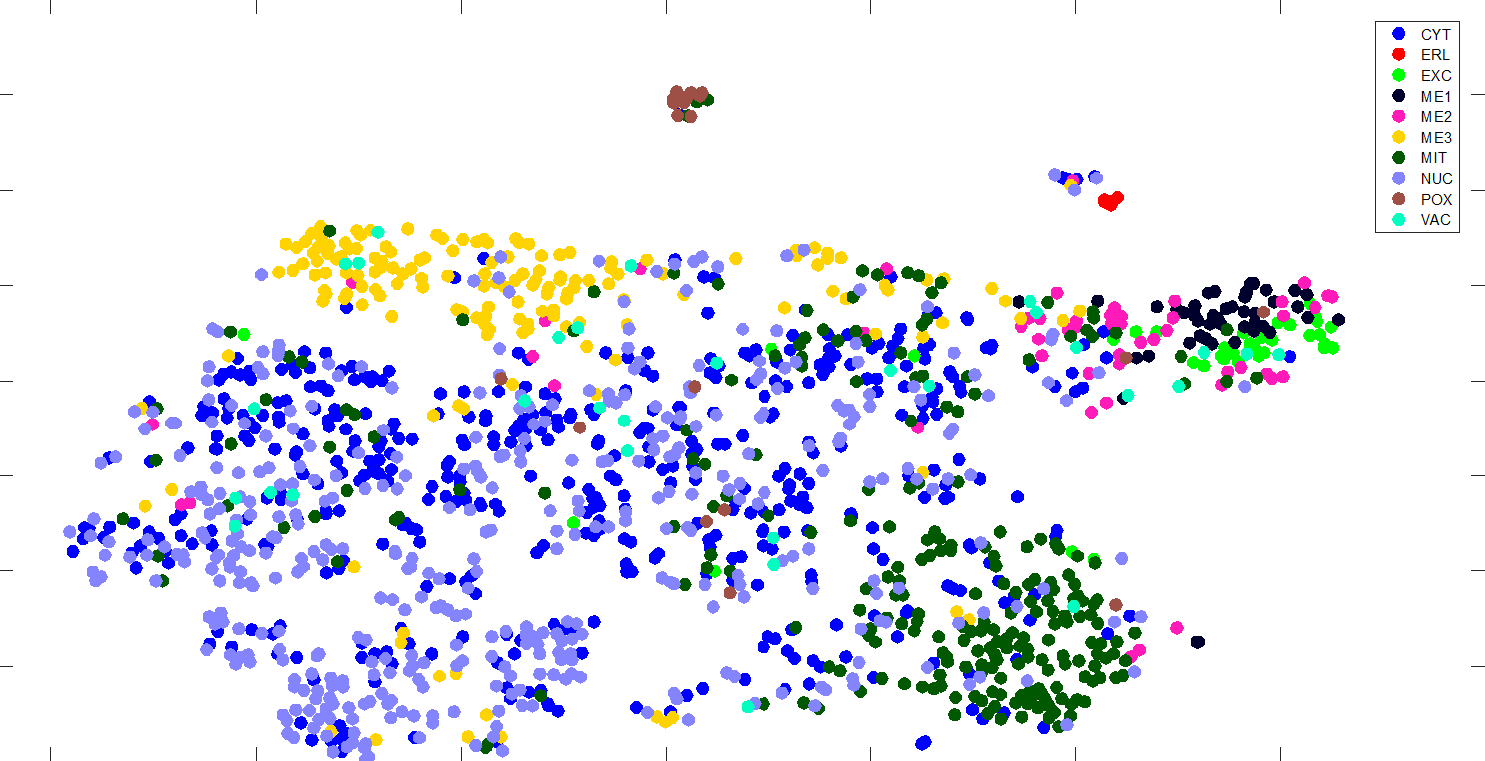
\includegraphics[width=0.9\linewidth]{figures/png/YeastTSNE}
	\caption[T-SNE visualization of Yeast dataset]{T-SNE visualization of Yeast dataset. Viewing in color is highly recommended.}
		\label{fig:yeasttsne}
\end{figure}



\paragraph{Cardiotocography Dataset}
Cardiotocography is the practice of monitoring fetal heartbeats during pregnancy.  The Cardiotocograph (CTG) is the machine used to monitor, and it produces cardiotocograms.    The dataset is based on \cite{ayres-de-campos_sisporto_2000} and was also used, in limited form, in \cite{ocak_medical_2013}, where the researchers achieved an impressive 100\% specificity (in this case, the correct classification of pathologic cardiotocograms).  Their sensitivity was also very high- 99.3\% on the training set.  Clearly here specificity is more important than sensitivity!  Unfortunately, these researchers left out approximately 200 samples of suspicious cardiotocograms, which confound things considerably.  There are good methodological reasons for doing this, of course- SVMs don't work as well with more than 2 classes, and culturally medicine is very concerned with sensitivity and specificity, which don't apply to non-binary problems in general.  We certainly aren't criticizing the good work medical researchers do, nor the lives they save.\\
We do include the suspect cardiotocograms, so we don't expect our results to be quite as clean. Further, there are two classification modes in this dataset, not 1.  The first is what we've mentioned already, the Normal, Suspect, Pathologic (NSP) classifications.  The second is the morphologic patterns 1-10.  These may or may not overlap with the NSP, but they provide a second way of looking at the data and evaluating it.  We have provided T-SNE visualizations with both colorings below in \ref{fig:cardio3tsne} and \ref{fig:cardio10tsne}.
\begin{figure}
	\centering
	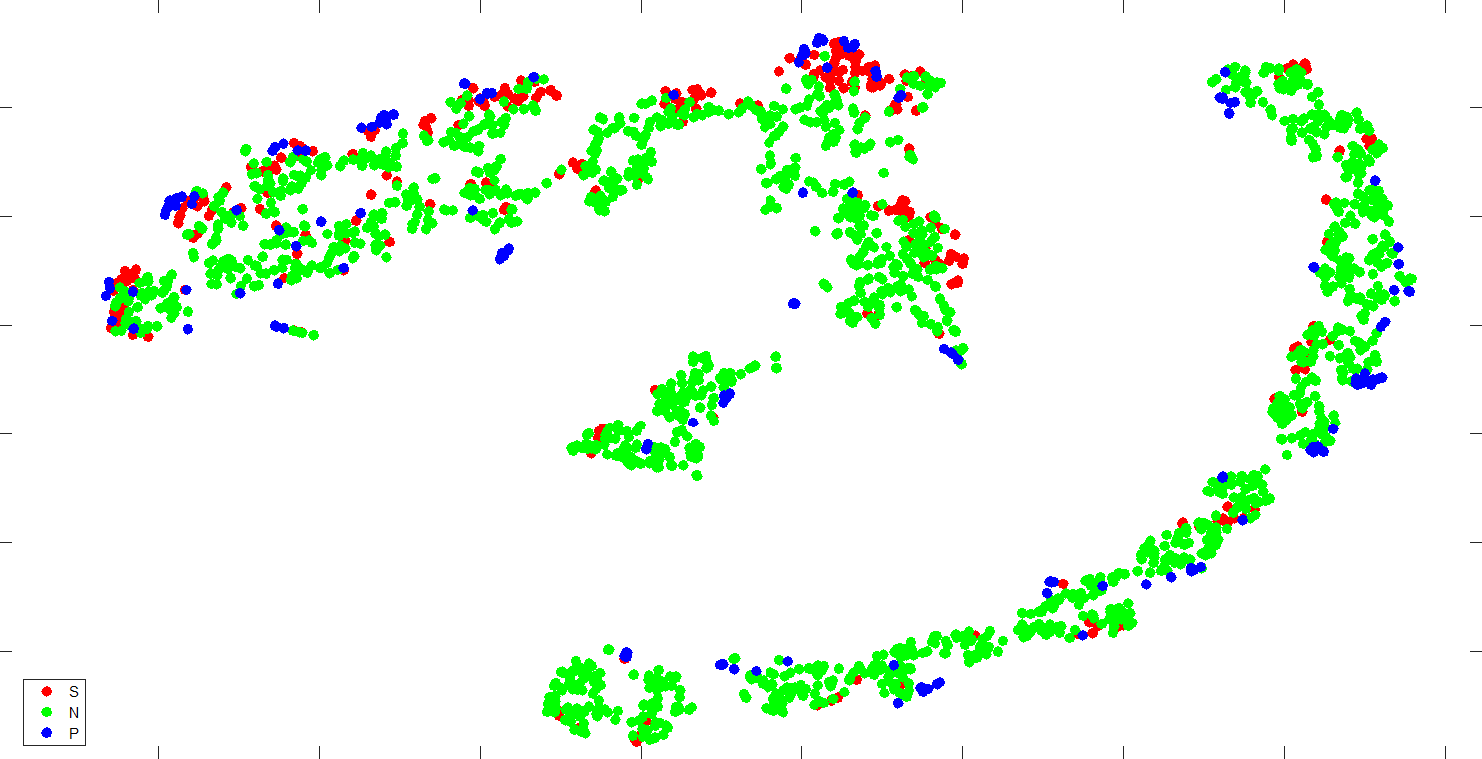
\includegraphics[width=0.9\linewidth]{figures/png/Cardio3TSNE}
	\caption[T-SNE visualization of Cardio dataset, NSP]{T-SNE visualization of Cardio dataset, following the NSP classification schema.}
	\label{fig:cardio3tsne}
\end{figure}
\begin{figure}
	\centering
	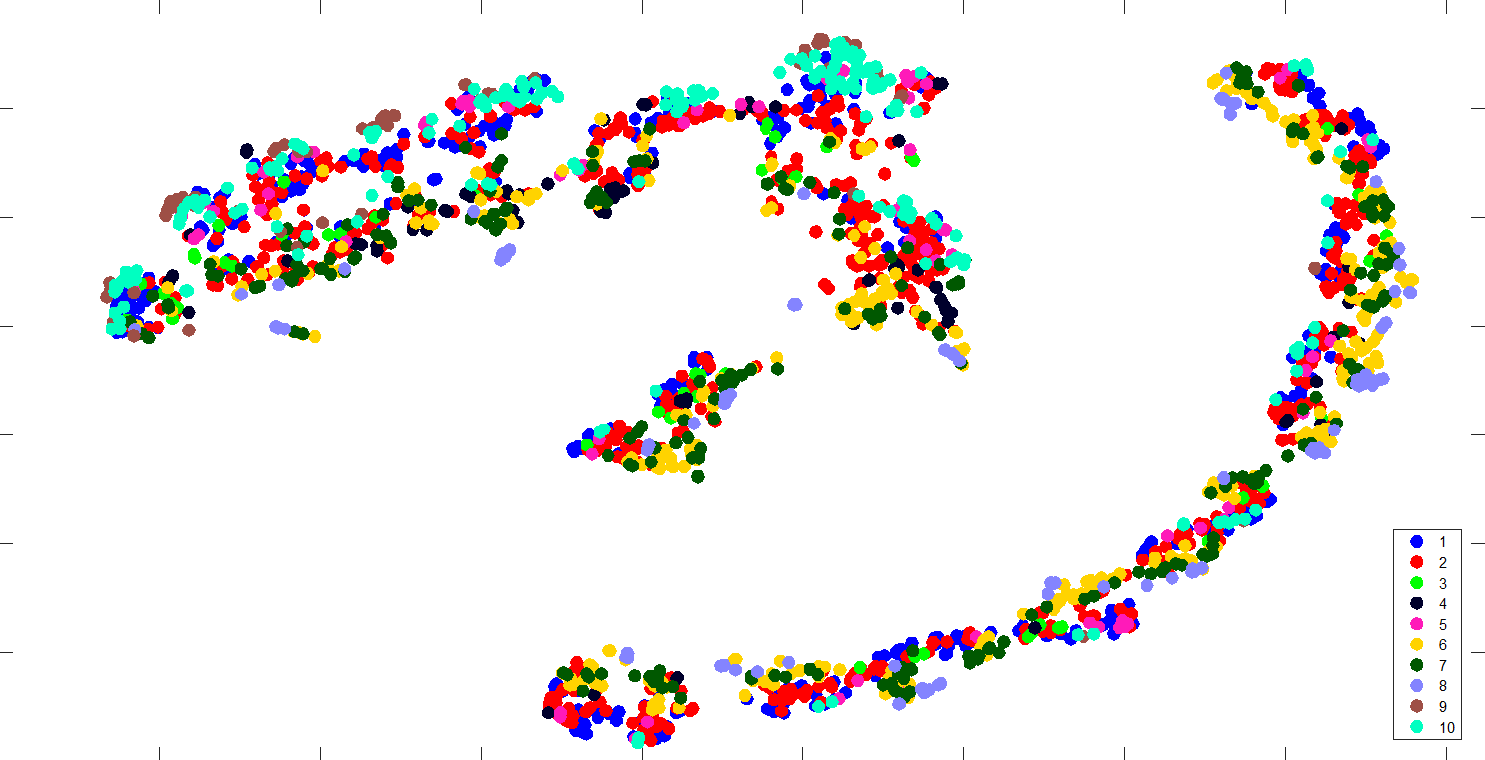
\includegraphics[width=0.9\linewidth]{figures/png/Cardio10TSNE}
	\caption[T-SNE visualization of Cardio dataset, morphology]{T-SNE visualization of Cardio dataset, following the 10-class morphology schema.  Viewing in color is highly recommended.}
	\label{fig:cardio10tsne}
\end{figure}
\paragraph{Bach's Chorales}
Bach composed all manner of music, but this dataset comprises 58 of his 4 part harmonies, called Chorales.  Originally made a dataset in \cite{radicioni_breve:_2010} the music of 58 chorales are painstakingly broken into 5665 musical moments, such that every time there are 3 or more distinct notes being played it their proper key is classified- but there are confounding factors. Primarily, there might be added notes, which means a note must always be taken in context, which makes the problem much more difficult.  What was a fairly modest 36 classes (12 notes $\times$ 3 modes) becomes 108 when added notes are taken into account.  Originally the authors used a perceptron which scored 75\% accuracy, which is certainly much better than chance because, while there are 108 possible classes, only 102 can actually be found in the dataset.  \\We should note that we modified this dataset slightly.  Initially they were published in the order in which they occurred.  We added an additional feature including the key of the previous event and then randomized the order of the file before splitting it into training and testing sets.  The hopes were that our algorithms would be able to take advantage of the temporal information in their models, even if they weren't explicitly instructed that it was temporal.  The visualization (\ref{fig:bachtsne}) is difficult to read because of the many classes, but clearly delineates several inherent clusters.
\begin{figure}
	\centering
	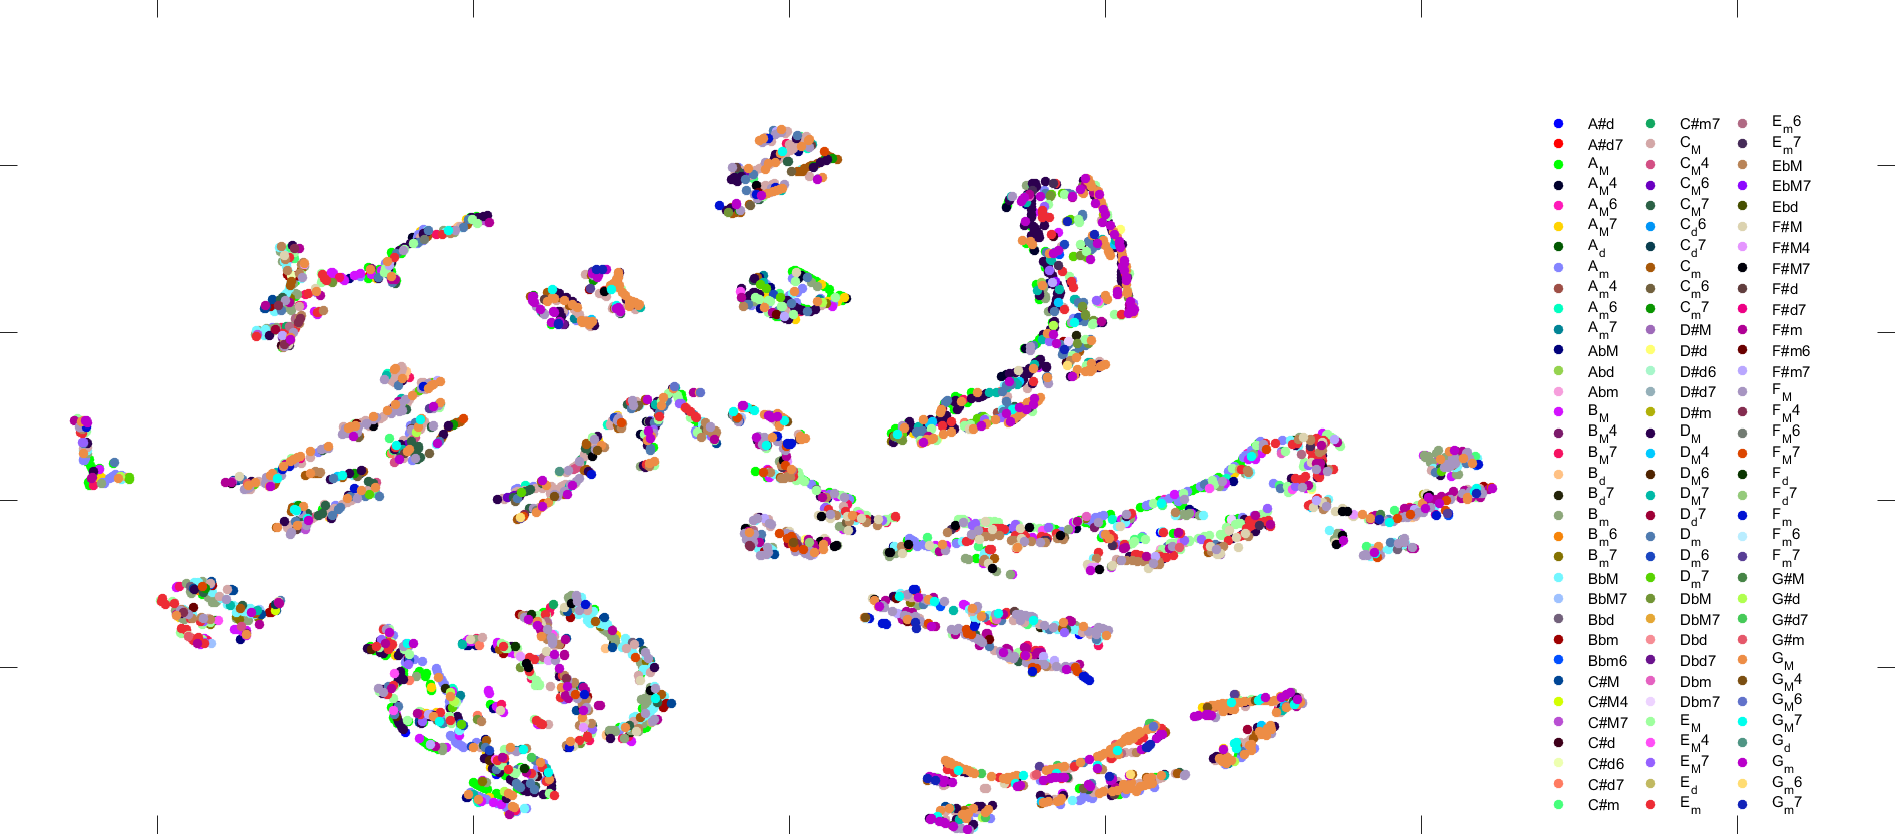
\includegraphics[width=0.9\linewidth]{figures/png/BachTSNE}
	\caption[T-SNE visualization of Bach dataset]{T-SNE visualization of 102 class Bach dataset.  Classes are incredibly difficult to distinguish, but instead focus on the overall shapes and distinct clusters.}
	\label{fig:bachtsne}
\end{figure}
\section{Results}
\subsection{Yeast}

\paragraph{CTree Baseline}:
As we can see, the baseline did fairly well regarding the 3 most common classes, but its ability to distinguish the less frequent classifications suffered giving it a final $\overline{A}$ of 64.1\%, or an overall accuracy of 74.6\%. See table \ref{tab:yeastctreebase} for more detail.\\
\begin{table}[h!]
\begin{tabular}{|c|c|c|c|c|c|c|c|c|c|c|c|}
\hline
Class&MIT&NUC&CYT&ME1&EXC&ME2&ME3&VAC&POX&ERL&Total
\\\hline
MIT&151&14&24&0&0&5&2&1&1&1&199\\
NUC&8&145&36&0&1&0&4&1&3&0&198\\
CYT&19&30&133&0&3&4&1&2&5&1&198\\
ME1&1&0&0&14&2&1&0&0&0&0&18\\
EXC&0&0&0&0&12&0&0&0&0&0&12\\
ME2&0&1&1&2&1&21&0&0&0&0&26\\
ME3&1&4&3&1&0&2&67&0&0&0&78\\
VAC&0&1&0&0&0&0&0&1&0&0&2\\
POX&0&0&1&0&0&0&0&0&5&0&6\\
ERL&0&0&0&0&0&0&0&0&0&3&3\\
\hline
Total:&180&195&198&17&19&33&74&5&14&5&740\\
TPR:&0.839&0.744&0.672&0.824&0.632&0.636&0.905&0.2&0.357&0.6&0.641\\
\hline
\end{tabular}
\caption[Yeast: Classification Tree without Feature Selection Confusion Matrix]{Yeast Dataset, Classification Tree with all features included, Accuracy = 74.6\%, MCC: 0.674 CEN: 0.273}
\label{tab:yeastctreebase}
\end{table}

\paragraph{CTree w/ feature selection}:
With feature selection $\overline{A}$ increased modestly to 65.8\%, but accuracy declined to 68.4\%.  See table \ref{tab:yeastctreefeatures}.\\  
\begin{table}[h]

\begin{tabular}{|c|c|c|c|c|c|c|c|c|c|c|c|}
	\hline
Class&MIT&NUC&CYT&ME1&EXC&ME2&ME3&VAC&POX&ERL&Total\\
MIT&131&13&9&0&0&1&2&0&2&0&158\\
NUC&8&87&26&0&1&0&1&2&0&0&125\\
CYT&33&87&158&0&3&2&4&2&4&0&293\\
ME1&1&0&0&13&2&1&0&0&0&0&17\\
EXC&1&0&0&1&11&1&0&0&0&0&14\\
ME2&5&2&1&2&2&26&0&0&0&1&39\\
ME3&1&5&3&1&0&2&67&0&0&0&79\\
VAC&0&1&0&0&0&0&0&1&0&0&2\\
POX&0&0&1&0&0&0&0&0&8&0&9\\
ERL&0&0&0&0&0&0&0&0&0&4&4\\
\hline
Total:&180&195&198&17&19&33&74&5&14&5&740\\
TPR:&0.728&0.446&0.798&0.765&0.579&0.788&0.905&0.2&0.571&0.8&0.658\\
\hline


\end{tabular}
\caption[Yeast: Classification Tree with Feature Selection Confusion Matrix]{Yeast Dataset, Classification Tree with feature selection, Accuracy = 68.4\%, MCC: 0.607 CEN: 0.290}
\label{tab:yeastctreefeatures}
\end{table}

\paragraph{McNB Baseline}
With all features, $\overline{A}$ was quite good: 85.9\%.  However, overall accuracy was 72.8\%.  See table \ref{tab:yeastctreebase} for confusion matrix and other details.
\\
\begin{table}[h!]
\begin{tabular}{|c|c|c|c|c|c|c|c|c|c|c|c|}
	\hline
Class&MIT&NUC&CYT&ME1&EXC&ME2&ME3&VAC&POX&ERL&Total\\\hline
MIT&119&10&10&0&0&0&1&0&1&0&141\\
NUC&9&108&17&0&0&1&0&0&0&0&135\\
CYT&18&35&152&0&1&0&0&1&0&0&207\\
ME1&4&4&2&17&0&0&0&0&0&0&27\\
EXC&4&6&2&0&18&0&0&0&0&0&30\\
ME2&12&9&5&0&0&32&2&0&0&0&60\\
ME3&8&10&5&0&0&0&71&0&0&0&94\\
VAC&1&5&0&0&0&0&0&4&0&0&10\\
POX&5&8&5&0&0&0&0&0&13&0&31\\
ERL&0&0&0&0&0&0&0&0&0&5&5\\
\hline
Total:&180&195&198&17&19&33&74&5&14&5&740\\
TPR:&0.661&0.554&0.768&1&0.947&0.97&0.959&0.8&0.929&1&0.859\\
\hline
\end{tabular}
\caption[Yeast: Multiclass Na\"ive Bayes without Feature Selection Confusion Matrix]{Yeast Dataset, Multiclass Na\"ive Bayes with all features included, Accuracy = 72.8\%, MCC: 0.671 CEN: 0.293}
\label{tab:yeastmcnbbase}
\end{table}

\paragraph{McNB w/ feature selection:}
With feature selection, Multiclass Na\"ive Bayes had the highest $\overline{A}$ of 87\%, though with an accuracy of only 72.8\%.  The disparity is accounted for in the accuracy across the first 3 classes, which make up more than $\frac{3}{4}$ of the dataset.  On them, accuracy ranged between abysmal and mediocre.  We can clearly see the danger of a highly skewed dataset and the dangers of metrics than are do not take this sufficiently into account.  See table \ref{tab:yeastctreebase} for details.
\\
\begin{table}[h!]
\begin{tabular}{|c|c|c|c|c|c|c|c|c|c|c|c|}
	\hline
Class&MIT&NUC&CYT&ME1&EXC&ME2&ME3&VAC&POX&ERL&Total\\
\hline
MIT&124&22&17&0&0&0&0&0&1&0&164\\
NUC&8&90&21&0&0&0&0&0&0&0&119\\
CYT&13&36&134&0&1&0&0&0&0&0&184\\
ME1&3&1&1&17&0&0&0&0&0&0&22\\
EXC&2&3&1&0&18&0&0&0&0&0&24\\
ME2&9&8&4&0&0&33&0&0&0&0&54\\
ME3&15&20&12&0&0&0&74&0&0&0&121\\
VAC&2&9&3&0&0&0&0&5&0&0&19\\
POX&4&5&5&0&0&0&0&0&13&0&27\\
ERL&0&1&0&0&0&0&0&0&0&5&6\\
\hline
Total:&180&195&198&17&19&33&74&5&14&5&740\\
TPR:&0.689&0.462&0.677&1&0.947&1&1&1&0.929&1&0.87\\
\hline
\end{tabular}
\caption[Yeast: Multiclass Na\"ive Bayes with Feature Selection Confusion Matrix]{Yeast Dataset, Multiclass Na\"ive Bayes with feature selection included, Accuracy = 72.8\%, MCC: 0.630 CEN: 0.310}
\label{tab:yeastmcnbfeatures}
\end{table}



	\paragraph{Hunter}
The Hunter underperformed the four other methods by any measure, and took a great deal (more than 100 times) more processor time to do it.  This was supposed to be the best case for the Hunters, and early indications say that it is.  $\overline{A}$ = .473\%, while accuracy is 51.1\%.  Table \ref{tab:yeasthunter}.
\\
	% TODO: Write writeup, interpret bits
\begin{table}[h!]
		\begin{tabular}{|c|c|c|c|c|c|c|c|c|c|c|c|}
		\hline
		Class&MIT&NUC&CYT&ME1&EXC&ME2&ME3&VAC&POX&ERL&Total\\
		\hline
MIT&105&17&12&0&0&0&0&0&0&0&134\\
NUC&2&37&10&1&0&1&3&0&0&0&54\\
CYT&43&94&142&0&5&3&2&1&10&0&300\\
ME1&4&1&0&8&1&3&7&0&0&0&24\\
EXC&9&2&3&0&9&7&0&0&2&0&32\\
ME2&1&9&6&6&4&12&1&1&0&2&42\\
ME3&14&5&11&2&0&6&58&1&0&0&97\\
VAC&2&28&13&0&0&1&3&2&0&0&49\\
POX&0&0&1&0&0&0&0&0&2&0&3\\
ERL&0&2&0&0&0&0&0&0&0&3&5\\
\hline
Total:&180&195&198&17&19&33&74&5&14&5&740\\
TPR:&0.583&0.19&0.717&0.471&0.474&0.364&0.784&0.4&0.143&0.6&0.473\\

		\hline
	\end{tabular}
	\caption[Yeast: Hunter]{Yeast Dataset, Hunter Accuracy = 51.1\%, MCC: 0.413 CEN: 0.409}
	\label{tab:yeasthunter}
\end{table}

Which classifier performed best is open for debate, both CTree and McNB are promising in their own ways.  CTree seems to do a better job with the bulk classes, and perhaps if you're optimizing average accuracy that's a good way to go- optimize a method for something it is less suited for, resulting in a kind of check on optimization gone awry.  Alternatively, perhaps the status of the major classes aren't as important, and the focus instead is on discriminating between the outlying classes.  In that case, McNB clearly wins.  In any case, the Hunter performed.  It didn't do well, exactly, and with more time it might have done better, but that applies to any of these methods.  The difference is that the Hunter already had 10 times as many generations and still didn't manage to get anywhere even close to competitive.

\subsection{Cardiotocography NSP}
\paragraph{CTree Baseline}
A classification tree handily gets 94\% accuracy on this dataset, but that will prove to be a fairly unsurprising given this dataset.  See table \ref{tab:cardioNSPctreebase} for more details.
\begin{table}[h!]
	\centering
	\begin{tabular}{|c|c|c|c|c|}
		\hline
		Class&Normal&Suspect&Pathologic&Total\\\hline
Normal&519&31&9&559\\
Suspect&12&408&0&420\\
Pathologic&10&0&74&84\\\hline
Total:&541&439&83&1063\\
TPR:&0.959&0.929&0.892&0.927\\
		\hline
	\end{tabular}
	\caption[Cardiotocography NSP: Classification Tree without Feature Selection Confusion Matrix]{Cardio Dataset, NSP Labels Classification Tree without feature selection included, Accuracy=94.1\%, MCC: 0.967 CEN: 0.043}
	\label{tab:cardioNSPctreebase}
\end{table}
\paragraph{CTree w/ Feature Selection}
With feature selection, we see a similar pattern to yeast.  Overall accuracy drops slightly, but the smaller classes get more accurate.  What's interesting here is that MCC and CEN both decrease; see table \ref{tab:cardioNSPctree} for more details.
\begin{table}[h]
	\centering
	\begin{tabular}{|c|c|c|c|c|}
		\hline
		Class&Normal&Suspect&Pathologic&Total\\\hline
Normal&514&34&3&551\\
Suspect&12&405&0&417\\
Pathologic&15&0&80&95\\\hline
Total:&541&439&83&1063\\
TPR:&0.95&0.923&0.964&0.946\\

		\hline
	\end{tabular}
	\caption[Cardiotocography NSP: Classification Tree with Feature Selection Confusion Matrix]{Cardio Dataset, NSP Labels Classification Tree with feature selection included, Accuracy: 93.9\% MCC: 0.962 CEN: 0.051}
	\label{tab:cardioNSPctree}
\end{table}

\paragraph{McNB Baseline}
We get an accuracy of 90.2\%, which is low compared to the previous classifiers, and the supporting metrics of MCC and CEN are much worse as well.  See table \ref{tab:cardioNSPmcnbbase} for details.
\begin{table}[h]
	\centering
	\begin{tabular}{|c|c|c|c|c|}
		\hline
Class&Normal&Suspect&Pathologic&Total\\\hline
Normal&476&24&6&506\\
Suspect&37&408&2&447\\
Pathologic&28&7&75&110\\\hline
Total:&541&439&83&1063\\
TPR:&0.88&0.929&0.904&0.904\\
\hline
	\end{tabular}
	\caption[Cardiotocography NSP: Multiclass Na\"ive Bayes without Feature Selection Confusion Matrix]{Cardio Dataset, NSP Labels Multiclass Na\"ive Bayes without feature selection included, Accuracy = 90.2\% MCC: 0.797 CEN: 0.186}
\label{tab:cardioNSPmcnbbase}
\end{table}
\paragraph{McNB w/ Feature Selection}
Here, McNB manages to redeem itself somewhat.  $\overline{A}$ is the highest for any of the classifiers, and accuracy is only slightly lower than the baseline CTree.  However, MCC and CEN are considerably worse than that tree- so take this classifiers' predictions with a grain of salt.  
\begin{table}[h]
	\centering
	\begin{tabular}{|c|c|c|c|c|}
		\hline
Class&Normal&Suspect&Pathologic&Total\\\hline
Normal&490&11&1&502\\
Suspect&28&427&0&455\\
Pathologic&23&1&82&106\\\hline
Total:&541&439&83&1063\\
TPR:&0.906&0.973&0.988&0.956\\
\hline
	\end{tabular}
	\caption[Cardiotocography NSP: Multiclass Na\"ive Bayes with Feature Selection Confusion Matrix]{Cardio Dataset, NSP Labels Multiclass Na\"ive Bayes with feature selection included, Accuracy = 94\%, MCC: 0.889 CEN: 0.116}
	\label{tab:cardioNSPmcnb}
\end{table}

\paragraph{Hunter}
This is probably the best we will see from the Hunter.  That said, it didn't do very well for the purpose of the dataset, which is distinguishing pathologic patterns from safe ones.  See table \ref{tab:cardioNSPHunter} for further discussion.

\begin{table}[h!]
	\centering
	\begin{tabular}{|c|c|c|c|c|}
		\hline
		Class&Normal&Suspect&Pathologic&Total\\\hline
Normal&197&77&10&284\\
Suspect&183&322&4&509\\
Pathologic&161&40&69&270\\\hline
Total:&541&439&83&1063\\
TPR:&0.364&0.733&0.831&0.643\\
		\hline
	\end{tabular}
	\caption[Cardiotocography NSP: Hunter Confusion Matrix]{Cardio Dataset, NSP Labels Hunter, Accuracy = 55\%, MCC: 0.333 CEN: 0.568}
	\label{tab:cardioNSPHunter}
\end{table}

As we can see, the CTree without feature selection performed best on this dataset.  For one thing, the dataset was developed by experts and they selected features that would be most indicative of problems.  Also, it might seem strange that MCC and CEN were so much lower on the Bayesian classifiers.  In examining the tables, pay close attention to how well the total in the right column matches the total in the row, and that should give an idea of why.  In some sense, MCC and CEN are measures of the useful information from the classifier.  In this case, when it makes a prediction of a particular class it's extremely confident.  That's much more useful than what the Bayesian classifiers discern, \textit{even though they get more of the pathological cases correct}.  Because even though the McNB with feature selection gets 82 of the 83 pathological cases, it also misclassified them about 20\% of the time. 
\subsection{Cardiotocography Morphology}
\paragraph{CTree Baseline}  
Again, this dataset proves to be highly separable, and CTree continues to do quite well.  See table \ref{tab:cardiomorphctreebase} for details. 
\begin{table}[h!]
	\centering
	\begin{tabular}{|c|c|c|c|c|c|c|c|c|c|c|c|}
	\hline
		Class&J&F&A&H&G&B&D&I&E&C&Total\\
\hline
		J&97&0&2&0&0&0&0&0&2&0&101\\
		F&0&159&0&1&5&6&0&0&0&0&171\\
		A&4&0&183&0&0&5&0&0&1&1&194\\
		H&0&0&0&42&2&0&1&0&0&2&47\\
		G&0&1&1&0&120&1&0&0&0&0&123\\
		B&0&0&1&0&0&286&3&0&3&1&294\\
		D&0&1&0&0&0&1&38&0&0&0&40\\
		I&3&0&1&0&0&0&0&28&0&0&32\\
		E&2&0&5&0&0&1&0&0&31&1&40\\
		C&0&0&2&0&0&0&0&0&0&19&21\\\hline
		Total:&106&161&195&43&127&300&42&28&37&24&1063\\
		TPR:&0.915&0.988&0.938&0.977&0.945&0.953&0.905&1&0.838&0.792&0.925\\
		\hline
	\end{tabular}
	\caption[Cardiotocology Morphology: Classification Tree  Confusion Matrix]{Cardio Dataset, Morphological Labels Classification Tree without feature selection included, Accuracy = 94.3\% MCC: 0.933, CEN: 0.086}
	\label{tab:cardiomorphctreebase}
\end{table}

\paragraph{CTree w/ Feature Selection}
Compared to the baseline, accuracy increased marginally but MCC got slightly worse.  CEN stayed the same to 3 significant figures.  See table \ref{tab:cardiomorphctree}.
\begin{table}
	\centering	
	\begin{tabular}{|c|c|c|c|c|c|c|c|c|c|c|c|}
	\hline
	Class&J&F&A&H&G&B&D&I&E&C&Total\\
	\hline
	J&98&0&0&0&0&0&0&0&2&1&101\\
	F&0&161&1&1&1&7&0&0&0&0&171\\
	A&6&0&178&0&0&4&0&1&3&2&194\\
	H&0&0&2&44&0&0&1&0&0&0&47\\
	G&0&4&1&0&118&0&0&0&0&0&123\\
	B&0&1&3&0&0&283&3&0&4&0&294\\
	D&0&1&0&0&0&0&39&0&0&0&40\\
	I&3&0&0&0&0&0&0&29&0&0&32\\
	E&1&0&5&0&0&0&0&0&33&1&40\\
	C&0&0&2&0&0&0&0&0&0&19&21\\\hline
	Total:&108&167&192&45&119&294&43&30&42&23&1063\\
	TPR:&0.907&0.964&0.927&0.978&0.992&0.963&0.907&0.967&0.786&0.826&0.922\\
	\hline
\end{tabular}
	\caption[Cardiotocology Morphology: Classification Tree Confusion Matrix]{Cardio Dataset, Morphological Labels Classification Tree with feature selection included accuracy: 94.3\% MCC: 0.931, CEN: 0.086}
	\label{tab:cardiomorphctree}
\end{table}
\paragraph{McNB Baseline}
Here, we again see the discriminative power of the Bayesian method- accuracy is up to 96\% and CEN is down a full 3.5 points and MCC is up by almost the same.  There's one class, I, where 100\% of the cases were caught, that is, one perfect column, though there's no corresponding perfect row.  See table \ref{tab:cardiomorphmcnbbase}.
\begin{table}[h!]
	\centering
	\begin{tabular}{|c|c|c|c|c|c|c|c|c|c|c|c|}
\hline
Class&J&F&A&H&G&B&D&I&E&C&Total\\
\hline
J&99&0&2&0&0&0&0&0&0&0&101\\
F&0&169&0&0&0&1&0&0&0&1&171\\
A&2&0&189&0&0&2&0&0&0&1&194\\
H&0&0&0&47&0&0&0&0&0&0&47\\
G&0&1&0&1&121&0&0&0&0&0&123\\
B&0&5&9&0&2&276&1&0&1&0&294\\
D&0&0&0&0&0&0&40&0&0&0&40\\
I&2&0&0&0&0&0&0&30&0&0&32\\
E&2&0&0&0&0&0&0&0&38&0&40\\
C&0&0&0&0&0&0&0&0&0&21&21\\\hline
Total:&105&175&200&48&123&279&41&30&39&23&1063\\
TPR:&0.943&0.966&0.945&0.979&0.984&0.989&0.976&1&0.974&0.913&0.967\\
\hline
	\end{tabular}
	\caption[Cardiotocography Morphology:  Na\"ive Bayes without Feature Selection Confusion Matrix]{Cardio Dataset Morphological Labels Multiclass Na\"ive Bayes without feature selection, Accuracy= 96.9\% MCC: 0.963, CEN: 0.05}
	\label{tab:cardiomorphmcnbbase}
\end{table}
\paragraph{McNB w/ Feature Selection}
This is the best we'll likely see from McNB: there are 3 perfect columns and 3 rows, and they overlap on 2 of the classes (I and H).  Accuracy and $\overline{A}$ are 98.3 and 98.1\%, respectively, MCC is 0.980 and CEN is 0.030.  See table \ref{tab:cardiomorphmcnb} for further details.
\begin{table}[h!]
	\centering
	\begin{tabular}{|c|c|c|c|c|c|c|c|c|c|c|c|}
		\hline
	Class&J&F&A&H&G&B&D&I&E&C&Total\\
	\hline
	J&100&0&1&0&0&0&0&0&0&0&101\\
	F&0&171&0&0&0&0&0&0&0&0&171\\
	A&0&0&187&0&1&4&0&0&1&1&194\\
	H&0&0&0&47&0&0&0&0&0&0&47\\
	G&0&1&0&0&122&0&0&0&0&0&123\\
	B&0&4&2&0&1&285&1&0&1&0&294\\
	D&0&0&0&0&0&0&40&0&0&0&40\\
	I&0&0&0&0&0&0&0&32&0&0&32\\
	E&0&0&0&0&0&0&0&0&40&0&40\\
	C&0&0&0&0&0&0&0&0&0&21&21\\
\hline
	Total:&100&176&190&47&124&289&41&32&42&22&1063\\
	TPR:&1&0.972&0.984&1&0.984&0.986&0.976&1&0.952&0.955&0.981\\
	
		\hline
	\end{tabular}
	\caption[Cardiotocography Morphology:  Na\"ive Bayes without Feature Selection Confusion Matrix]{Cardio Dataset Morphological Labels Multiclass Na\"ive Bayes with feature selection, Accuracy = 98.3\%, MCC: 0.98, CEN: 0.03}
	\label{tab:cardiomorphmcnb}
\end{table}
\paragraph{Hunter}
This hunter actually manages a negative MCC, which represents it performing worse than chance. In some sense, this means that if this classifier says something you're better off picking \textit{anything else} at random.  See table \ref{tab:cardiomorphhunter} for details of its lackluster performance.  
\begin{table}[h!]
	\centering
	\begin{tabular}{|c|c|c|c|c|c|c|c|c|c|c|c|}
		\hline
		Class&J&F&A&H&G&B&D&I&E&C&Total\\\hline
		J&28&19&0&1&21&0&3&2&27&0&101\\
		F&0&5&0&0&2&163&1&0&0&0&171\\
		A&16&86&10&0&33&5&1&40&1&2&194\\
		H&0&1&0&38&4&3&0&1&0&0&47\\
		G&0&43&0&1&65&3&10&1&0&0&123\\
		B&2&3&0&0&2&284&1&2&0&0&294\\
		D&0&0&0&0&0&40&0&0&0&0&40\\
		I&0&6&0&16&0&0&0&10&0&0&32\\
		E&9&7&0&0&12&0&0&8&4&0&40\\
		C&0&11&0&0&3&0&1&6&0&0&21\\\hline
		Total:&55&181&10&56&142&498&17&70&32&2&1063\\
		TPR:&0.509&0.028&1&0.679&0.458&0.57&0&0.143&0.125&0&0.351\\
		\hline
	\end{tabular}
	\caption[Cardiotocography Morphology: Hunter Confusion Matrix]{Cardio Dataset Morphological Labels Multiclass Na\"ive Bayes with feature selection, Accuracy = 41.7\%, MCC: -0.078, CEN: 0.49}
	\label{tab:cardiomorphhunter}
\end{table}


\subsection{Bach's Chorales}
Unfortunately, there's not a good way of fitting a 103 index square confusion matrix on a single page that preserves readability.  Thus, we have included instead copies of excel spreadsheets with the relevant data in our attachments.  We will discuss them as normal.


\paragraph{CTree Baseline}
	CTree had some difficulty with this dataset.  MCC was decent at 0.694, CEN seemed to be relatively good at 0.18.    However, accuracy was 70.9\%, which seems like decent performance (the perceptron in the original paper got 75\%, after all), and the MCC seems to indicate this result is from some consolidation of signal rather than chance.  $\overline{A}$ is very low at 24.4\%, but with so many classes that is not particularly surprising.  
\paragraph{CTree w/ Feature Selection}	
Unusually, performance decreased by most metrics here.  That might be indicative that all dimensions are important to this set, which makes sense for music- it would be hard to discern the difference between two chords if you ignore a single key which contributes to one and not the other.  This pattern doesn't hold with the Bayesian classifier.  Accuracy is 67.9\%, while $\overline{A}$ is 27.0\%.    MCC was 0.662, and CEN was 0.192.
\paragraph{McNB Baseline}
Here, we see a marked difference in performance between CTree and McNB.  MCC at 0.785 is noticeably higher, and CEN at 0.139 is lower by about the same margin, and accuracy beats the original paper at 79.4\%.  $\overline{A}$ is the biggest difference, though, and nearly triples the baseline CTree's result at 66.2\%.
\paragraph{McNB w/ Feature Selection}
This optimizer performs comparably to the baseline, being slightly better in MCC (0.794), CEN(0.136) and Accuracy(80.3\%), but coming in slightly under in $\overline{A}$ at 65.3\%.  
\paragraph{Hunter}
Due to numerous troubles getting the Hunters to run on this dataset, we still don't have results from more than a few dozen generations.  To be added as we get them.  Our 1,925 generation run, which took 3 weeks, resulted in an MCC of 0.196, and a CEN of 0.307, which is better than random.  However, because the training set was missing a handful of the more rare classes, it isn't an apples-to-apples comparison.  We'll update this with whatever we can gather from our current run, which is up to 15 generations at the time of writing.

\section{Final Thoughts}
\begin{figure}
	\centering
	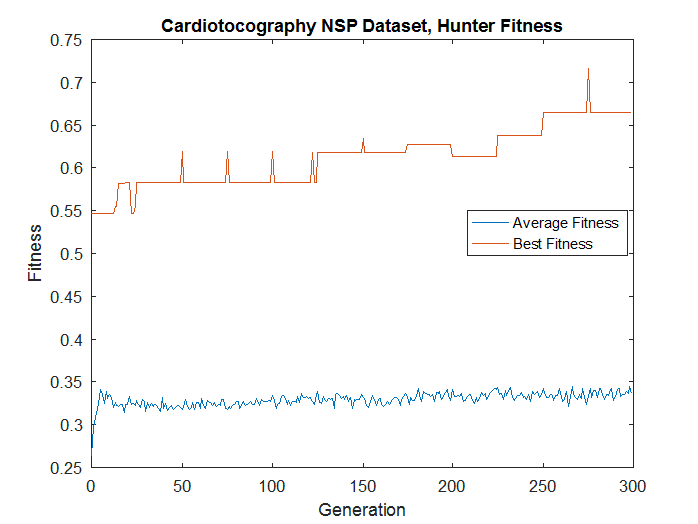
\includegraphics[width=0.7\linewidth]{figures/png/fitnessCardioNSPHunter}
	\caption[Hunter Population Growth, CardioNSP]{This figure demonstrates Hunter fitness, average and best, over the lifespan of a trial, in this case 300 generations. Where there seems to be lacking monotonicity is actually the result of validation fitness, which has the best Hunters seemingly scoring much better on the testing set.}
	\label{fig:fitnesscardionsphunter}
	
	\includegraphics[width=0.7\linewidth]{figures/png/fitnessCardioNSPMcNB}
	\caption[Multiclass Na\"ive Bayes Optimizer Growth, CardioNSP]{
	Population fitness of the McNB Optimizer on the CardioNSP dataset.  This overall shape is typical of most Optimizers.}
	
\end{figure}

It is clear that theoretically based algorithms are better at solving problems than trying to co-opt a GA to do it on its own.  
As for whether we should use McNB or CTree, the answer is clear: neither.  We've already written far better performing algorithms elsewhere, including aggregate trees and support vector machine optimizers.  The purpose of those algorithms was to give Hunters competition that wouldn't completely outclass them, and they failed in that regard.  This is at least partially because Na\"ive Bayes is such a robust first pass, and there are good reasons to use it in ensemble methods because it does such a good job extracting signal from messy data.  Further, it does a decent job differentiating classes with few samples.\\
The most surprising performance was from CTree- while we have used trees in aggregate before, they performed far better alone than expected, in some regards holding their own up against Na\"ive Bayes, though mostly in terms of overall accuracy and only if we're being accommodating.  Still, their performance was better than we would have expected going into the project.\\
Hunters performed poorly.  There might be some way of improving their performance, which we've noted as we've gone through the document.  However, there should be a case made that such an endeavor is worthwhile, and one would need significant data contradicting this paper to say that there remains a compelling reason to do so.  When we began this project, we believed that they had a decent chance to at least hold their own with our methods.  This has been proven to be false across numerous comparisons.  Further, we ``cheated" on behalf of the Hunter, giving it vast additional resources, time, and modified starting conditions.  We gave it every advantage, and it failed to deliver.  The evidence is not conclusive for genetic algorithms in general, but this GA specifically is vastly inferior to even modest hybrid classification methods and should be retired.  
    \chapter{Conclusions} \label{ch:conclusion}
Genetic Algorithms should probably be used to optimize rather than classify.  Without considerably more work developing a better algorithm to create an extensible generic universal genetic classifier, there's simply too much theoretical ground to make up.  GAs still do a good job optimizing, and can get the same or better performance out of them, which is very similar to the real evolution.  This project felt like forcing a speedboat to race against kittens piloting a bucket, and then being shocked as even without any other advantages the speedboat won every time.\\In the end, evolutionary algorithms are a swiss-army knife.  Certainly, a GA would be able to solve linear programming problems better than a support vector machine, but that isn't even in the realm of a fair comparison.  GAs are good at what they do- optimizing a fitness function over time in a way that resembles evolution.  They can easily be overwhelmed with genomes of great length, which is one area where real evolution has a huge edge.  First, it is massively and embarrassingly parallel.  Second, developmental biology is great at branch and bound.  In other words, genomes that will have trouble producing viable solutions will themselves be less likely to exist because of many pass or fail tests along the way.  Oh, and it also has a billion years or more to come up with solutions.  If there were a way for GAs to take advantage of additional parallelism or checkpoints that might be a place for further research.  Another place might be in finding similarly generic tools which we could leverage, like, perhaps, neural nets to take a first pass at a dataset and then using a Hunter-like approach to distinguish results- though, if neural nets are already involved, there would need to be a good reason to invoke a Hunter when some other neural net would likely get better results, especially given their lackluster performance here.  One reason for using Hunters despite their mediocre performance they are extremely transparent: a Hunter will distill its decision making into unambiguous rules (even if it is a slew of them), where a neural net by its nature relies on numerous hidden calculations.  This transparency was a major motivating factor for this approach to begin with.\\
Some other direction that might be worth pursuing is finding a way to combine more theoretical underpinnings with a GA.  For instance, here the mechanics available to the Hunter were somewhat lackluster.  All they could do were make boolean decisions based on the absolute values of features.  That's simply not enough for modern datasets.  As mentioned, GAs are extremely good at leveraging tools given to them and combining them in interesting ways, so one might consider improving the quality of the toolbox a useful avenue for further research. This could be branching on any number of concepts, including statistical ones or neural network inspired, or perhaps abandoning ensemble voting altogether and coming to some conclusion more akin to maximum likelihood estimation.  An example of that might be building different PDFs for each class from an arbitrary number of Gaussian functions and evaluating based on the resulting metrics.\\
$\overline{A}$ has proved to be a flawed metric, as to some degree all metrics are. We would still argue that it is less flawed than anything simpler.  Until this result, our findings with $\overline{A}$ is that it was usually $\approxeq$ to accuracy.    Here, however, whether because of the skew of the datasets or some other confounding factor, $\overline{A}$ was often very different from raw accuracy, which is a place for either further research or a reason to find a new metric. In hindsight, and even from an \textit{a priori} standpoint, it seems obvious that if you only consider the diagonal of a confusion matrix you're losing useful information.  \cite{jurman_comparison_2012} includes a few methods which might be valuable for multi-class confusion matrices.     Matthew's Correlation Coefficient and Confusion Entropy seem promising, and implementing them as a fitness function would be fairly straightforward.   We calculate these metrics for the classifications we have already gathered, however future work might include using one or a weighted combination of both as better metrics for scoring multi-class classifiers.
\\ 
The optimizers performed well, given relatively very few generations.  The next area of research for them is combining them and connecting their outputs back into another optimizer for a difficult or intractable dataset, combining them in novel ways to get the maximum signal from a dataset, perhaps even a meta-optimizer that will optimize an ensemble of disparate optimizers, themselves optimizing primitive classifiers.  That seems like a promising way of limiting the search length for each population of optimizers while still searching a much larger space, though more research would be needed to show that it is viable.  For instance, the meta-optimizer could have a few bits for each subordinate optimizer, probably of different types.  The first section of the bits would encode two numbers, the first for how many optimizers to train and the second for how many features to include.   Then, the subordinate optimizers would operate under the constraint of including no more than the number of features, and would separately and quickly evolve an ensemble of different classifiers.  These classifiers in turn would provide their output to the meta-optimizer who would then optimize a classifier of its own using all the features and the classifications made by its ensemble of classifiers as a new table.  This might be feasible given the speed with which many of the classifiers were able to evolve, and the robustness of the classifiers generated in such a manner.\\

    %%%%%%%%%%%%%%%%%%%%%%%%%%%%%%%%%%%%%%%%%%%%%%%%%%%%%%%%%%%%%%%%%%%%%%%%%%%%%%%%%%%%%%%%%%%%%%%%%%%%%
    % BIBLIOGRAPHY
    %%%%%%%%%%%%%%%%%%%%%%%%%%%%%%%%%%%%%%%%%%%%%%%%%%%%%%%%%%%%%%%%%%%%%%%%%%%%%%%%%%%%%%%%%%%%%%%%%%%%%
    \makeBibliographyPage % make the bibliography title page - can be edited in ut-thesis-template.tex
    \bibliographystyle{apalike} % bibliography style - recommend using apalike-doi as it hyperlinks DOIs
    \bibliography{references/references-dissertation} % references.bib included in the references directory
    %%%%%%%%%%%%%%%%%%%%%%%%%%%%%%%%%%%%%%%%%%%%%%%%%%%%%%%%%%%%%%%%%%%%%%%%%%%%%%%%%%%%%%%%%%%%%%%%%%%%%
    % APPENDIX - OPTIONAL - COMMENT IF NOT NEEDED
    %%%%%%%%%%%%%%%%%%%%%%%%%%%%%%%%%%%%%%%%%%%%%%%%%%%%%%%%%%%%%%%%%%%%%%%%%%%%%%%%%%%%%%%%%%%%%%%%%%%%%
    \makeAppendixPage   % make the appendix title page - can be edited in ut-thesis-template.tex
    \appendix
    \chapter{Hunter Genomes and Explanations}
\section{Yeast}
	\begin{tabular}{|c c c c c c c|}
		\hline
	&Aff & Cla & Not & Cell 1 &Cell 2&\\
	\hline
	&01&0111& 1 &100000000110010111011&&\\
	&11&0101& 1 &111011011100111100001&&\\
	&11&0001& 0 &010001100101111101011&&\\
	&10&0011& 1 &001001100110111010100&&\\
	&11&0000& 1 &110110101001110001001&&\\
	&10&0010& 1 &001101100010111101110&&\\
	&11&0101& 1 &000000101001110111000&110100101110001110100&\\
	&00&0110& 0 &101001101001111001101&011000001011011101010&\\
	&11&0100& 1 &000000011000101010111&&\\
	&11&1000& 1 &000010101001110110011&&\\
	&11&0001& 0 &011101101011111010011&&\\
\end{tabular} \\cont'd\\\\\pagebreak[4]
\begin{tabular}{|c c c c c c c|}
\hline
&Aff & Cla & Not & Cell 1 &Cell 2&\\
\hline	
	&10&1000& 0 &010101011011101011101&110010011111101111101&\\
	&01&1001& 0 &100000101110100110111&&\\
	&00&0000& 0 &001101011000110010110&&\\
	&01&1001& 1 &000100111111101101111&&\\

	&11&0001& 1 &001100011001101010100&&\\
	&01&0111& 0 &000100001000010010110&&\\
	&11&0101& 0 &100000110011101111101&&\\
	&01&0100& 0 &011110110001111111001&&\\
	&10&0011& 1 &000100110000101101001&&\\
	&01&0011& 0 &011101011101110101010&&\\
	&11&0100& 1 &111001100000110101010&&\\
	&01&0001& 0 &011101011001110000101&&\\
	&01&0111& 1 &011001100101110111001&&\\
	\hline
\end{tabular}


\begin{lstlisting}[caption={Best Hunter, Yeast}]
This hunter has the following 24 chromosomes:
This chromosome prefers the rear
It focuses on problems in the following class:
VAC
By aggregating the nay votes from the following 1 cell:
This cell looks at feature 0
whose return value is between 0.0234375 and 0.36328125 

This chromosome considers itself complete
It focuses on problems in the following class:
ME2
By aggregating the nay votes from the following 1 cell:
This cell looks at feature 6
whose return value is between 0.859375 and 0.9375 

This chromosome considers itself complete
It focuses on problems in the following class:
NUC
By aggregating the yes votes from the following 1 cell:
This cell looks at feature 4
whose return value is not between 0.39453125 and 0.95703125 

This chromosome prefers the front
It focuses on problems in the following class:
ME1
By aggregating the nay votes from the following 1 cell:
This cell looks at feature 2
whose return value is not between 0.3984375 and 0.9140625 

This chromosome considers itself complete
It focuses on problems in the following class:
MIT
By aggregating the nay votes from the following 1 cell:
This cell looks at feature 5
whose return value is between 0.66015625 and 0.765625 

This chromosome prefers the front
It focuses on problems in the following class:
CYT
By aggregating the nay votes from the following 1 cell:
This cell looks at feature 3
whose return value is not between 0.3828125 and 0.96484375 

This chromosome considers itself complete
It focuses on problems in the following class:
ME2
By aggregating the nay votes from the following 2 cells:
This cell looks at feature 0
whose return value is not between 0.16015625 and 0.859375 

This cell looks at feature 5
whose return value is between 0.1796875 and 0.2265625 

This chromosome has no preference
It focuses on problems in the following class:
ME3
By aggregating the yes votes from the following 2 cells:
This cell looks at feature 2
whose return value is between 0.41015625 and 0.8984375 

This cell looks at feature 6
whose return value is not between 0.04296875 and 0.45703125 

This chromosome considers itself complete
It focuses on problems in the following class:
EXC
By aggregating the nay votes from the following 1 cell:
This cell looks at feature 0
whose return value is not between 0.09375 and 0.66796875 

This chromosome considers itself complete
It focuses on problems in the following class:
POX
By aggregating the nay votes from the following 1 cell:
This cell looks at feature 0
whose return value is not between 0.66015625 and 0.84765625 

This chromosome considers itself complete
It focuses on problems in the following class:
NUC
By aggregating the yes votes from the following 1 cell:
This cell looks at feature 7
whose return value is not between 0.41796875 and 0.91015625 

This chromosome prefers the front
It focuses on problems in the following class:
POX
By aggregating the yes votes from the following 2 cells:
This cell looks at feature 5
whose return value is not between 0.35546875 and 0.6796875 

This cell looks at feature 4
whose return value is between 0.62109375 and 0.7421875 

This chromosome prefers the rear
It focuses on problems in the following class:
ERL
By aggregating the yes votes from the following 1 cell:
This cell looks at feature 0
whose return value is between 0.1796875 and 0.60546875 

This chromosome has no preference
It focuses on problems in the following class:
MIT
By aggregating the yes votes from the following 1 cell:
This cell looks at feature 3
whose return value is not between 0.34375 and 0.79296875 

This chromosome prefers the rear
It focuses on problems in the following class:
ERL
By aggregating the nay votes from the following 1 cell:
This cell looks at feature 1
whose return value is not between 0.24609375 and 0.71484375 

This chromosome considers itself complete
It focuses on problems in the following class:
NUC
By aggregating the nay votes from the following 1 cell:
This cell looks at feature 3
whose return value is not between 0.09765625 and 0.6640625 

This chromosome prefers the rear
It focuses on problems in the following class:
VAC
By aggregating the yes votes from the following 1 cell:
This cell looks at feature 1
whose return value is not between 0.03125 and 0.29296875 

This chromosome considers itself complete
It focuses on problems in the following class:
ME2
By aggregating the yes votes from the following 1 cell:
This cell looks at feature 0
whose return value is between 0.19921875 and 0.7421875 

This chromosome prefers the rear
It focuses on problems in the following class:
EXC
By aggregating the yes votes from the following 1 cell:
This cell looks at feature 7
whose return value is not between 0.69140625 and 0.984375 

This chromosome prefers the front
It focuses on problems in the following class:
ME1
By aggregating the nay votes from the following 1 cell:
This cell looks at feature 1
whose return value is not between 0.1875 and 0.703125 

This chromosome prefers the rear
It focuses on problems in the following class:
ME1
By aggregating the yes votes from the following 1 cell:
This cell looks at feature 7
whose return value is not between 0.36328125 and 0.83203125 

This chromosome considers itself complete
It focuses on problems in the following class:
EXC
By aggregating the nay votes from the following 1 cell:
This cell looks at feature 6
whose return value is between 0.375 and 0.83203125 

This chromosome prefers the rear
It focuses on problems in the following class:
NUC
By aggregating the yes votes from the following 1 cell:
This cell looks at feature 7
whose return value is not between 0.34765625 and 0.7578125 

This chromosome prefers the rear
It focuses on problems in the following class:
VAC
By aggregating the nay votes from the following 1 cell:
This cell looks at feature 6
whose return value is not between 0.39453125 and 0.859375 

\end{lstlisting}


\section{Cardio NSP}



\section{Cardio Morphology}



\section{Bach}
    %%%%%%%%%%%%%%%%%%%%%%%%%%%%%%%%%%%%%%%%%%%%%%%%%%%%%%%%%%%%%%%%%%%%%%%%%%%%%%%%%%%%%%%%%%%%%%%%%%%%%
    % A VITA IS REQUIRED
    %%%%%%%%%%%%%%%%%%%%%%%%%%%%%%%%%%%%%%%%%%%%%%%%%%%%%%%%%%%%%%%%%%%%%%%%%%%%%%%%%%%%%%%%%%%%%%%%%%%%%
    \addToTOC{Vita}
    \chapter*{Vita} \label{ch:vita}
Vita goes here...
\end{document}
